% !TEX TS-program = xelatex
% !TEX encoding = UTF-8


\documentclass{elsarticle}
\usepackage{amsmath,amssymb,amsfonts}
\usepackage{graphicx}

\usepackage{geometry}
\geometry{left = 1.5cm, right = 1.5 cm}

\begin{document}
\title{Investigation upon the performance of piezoelectric energy harvester with flexible extensions}
\author{Maoying Zhou, Weiting Liu}
\maketitle


\begin{abstract}
    hello I begin
\end{abstract}

\section{Model Description}

We seek to investigate the influence of a flexible extension upon the overall performance of a classic piezoelectric cantilever beam energy harvester. In our problem, the energy harvester is comprised of two parts: the primary beam part and the beam extension part, as shown in Figure~\ref{fig:fig_beam_configuration}.
\begin{figure}[!htbp]
    \centering
    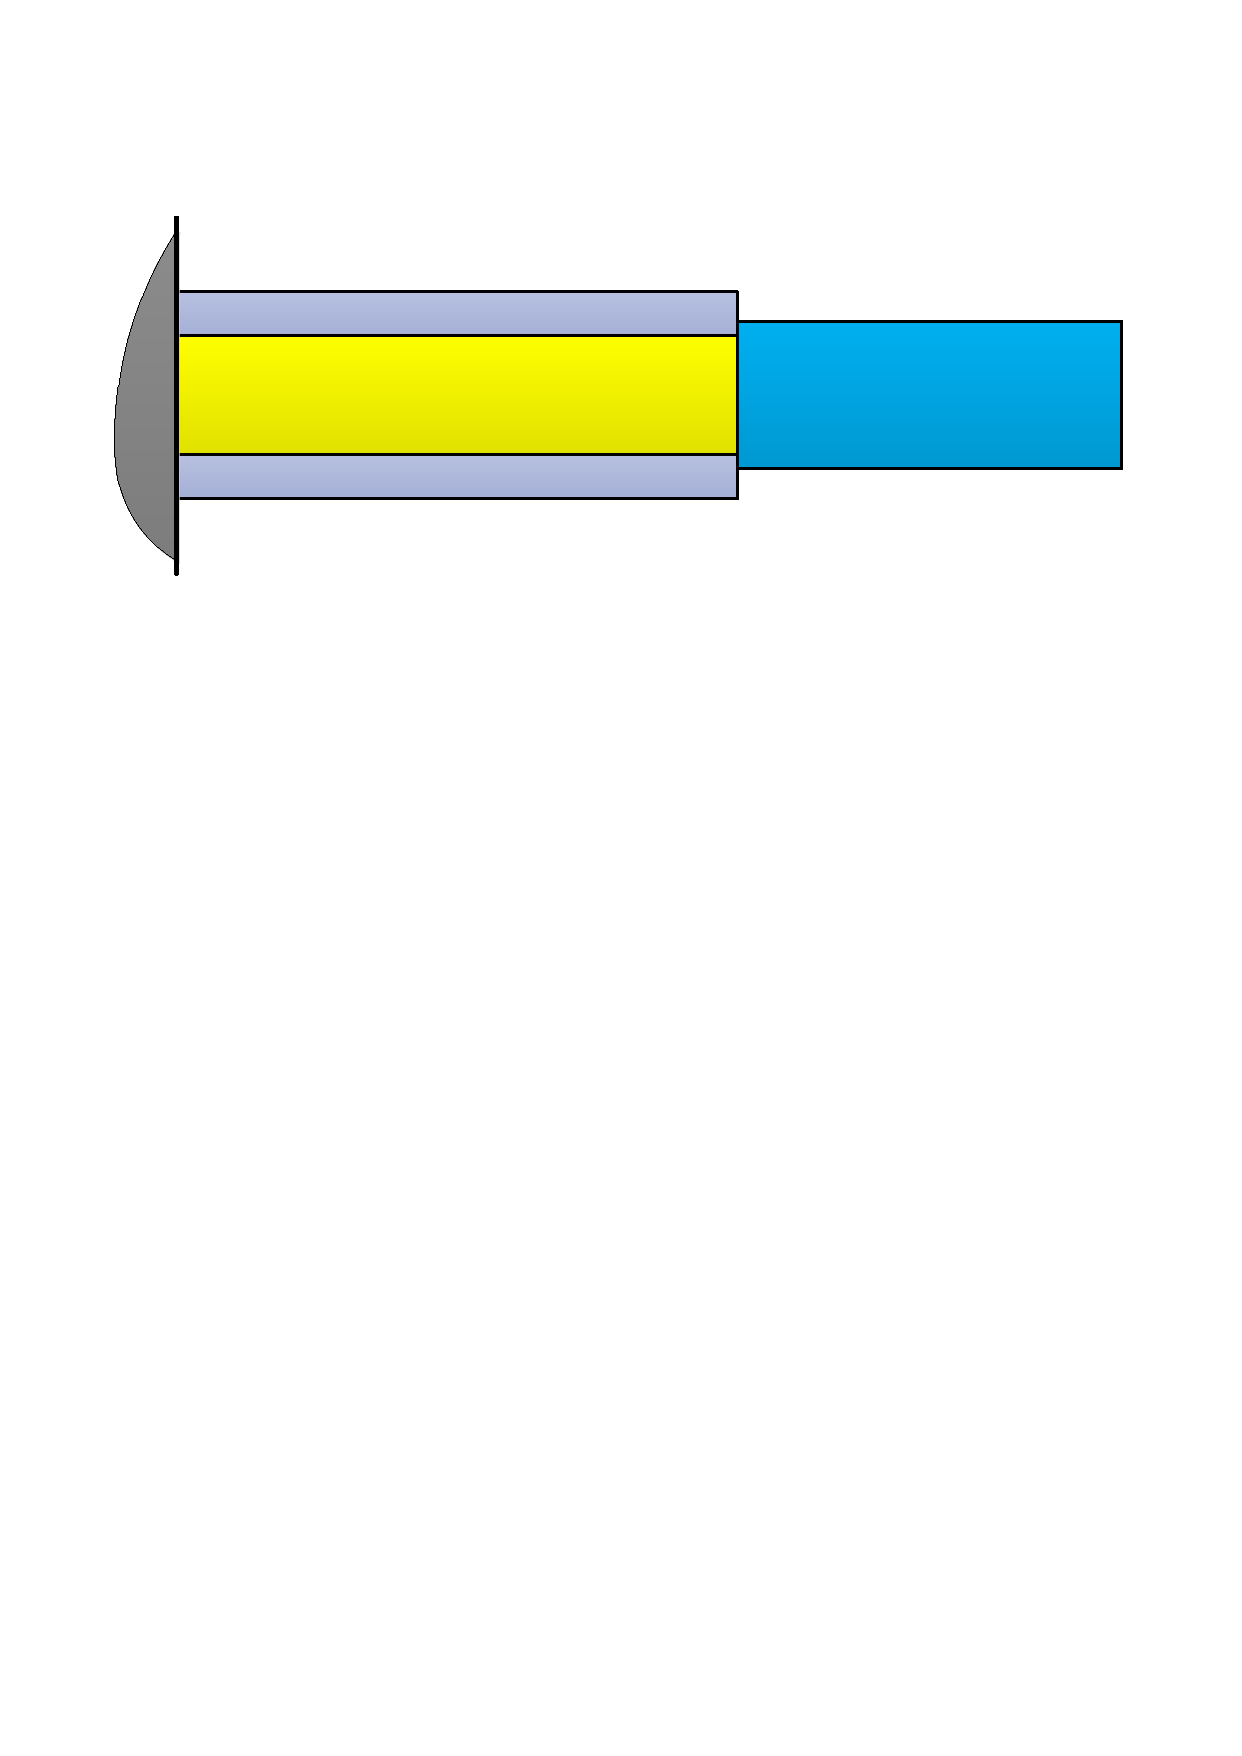
\includegraphics[width=0.8\textwidth]{./fig_beam_configuration.pdf}
    \caption{Schematic configuration of the piezoelectric energy harvester with flexible extension.}
    \label{fig:fig_beam_configuration}
\end{figure}

Following the classical analyzing process of piezoelectric bimorph cantilever beams \cite{erturk2009experimentally,park2003dynamics}, we can simply list the following dimensional equations for the piezoelectric primary beam part as:
\begin{equation}
    \left\{\begin{aligned}
        M_p(x_1,t) &= B_p \frac{\partial^2 w_1(x_1,t)}{\partial x_1^2} - e_p V_p (t) \\
        q_p(x_1,t) &= e_p \frac{\partial^2 w_1(x_1,t)}{\partial x_1^2} + \epsilon_p V_p (t),
    \end{aligned}\right.
\end{equation}
where where $M_p(x_1,t)$ is the moment at cross section of $x_1$ and $q_p(x_1,t)$ is the corresponding line charge density on the electrode. $w_1(x_1,t)$ is the displacement function of the primary beam part with $0 \leq x_1 \leq l_p$ and $V_p(t)$ is the voltage across the electrodes. The corresponding coefficients $B_p$, $e_p$, and $\epsilon_p$ are defined as
\begin{equation}
    B_p = \frac{2}{3}b\left\{ E_s h_s^3 + c_{11}^E \left[ (h_s+h_p)^3 - h_s^3 \right] \right\}, \quad e_p = b e_{31}\left(h_s+\frac{1}{2}h_p\right), \quad \epsilon_p = \frac{b \epsilon_{33}^S}{2 h_p}
\end{equation}
in which $c_{11}^E$ and $E_s$ are the elastic constants of the piezoelectric layer and the structure layer, respectively, $e_{31}$ is the piezoelectric charge constant of the piezoelectic layer, $\epsilon_{33}^S$ is the dielectric constant of the piezoelectric layer, $h_s$ and $h_p$ are the half structure layer thickness and piezoelectric layer thickness, respectively, $l_p$ is the length of the primary beam part, and $b$ is the width of the primary beam part.

In terms of the mechanical balance, the equation of a piezoelectric beam can be established using the Euler-Bernoulli assumptions as follows
\begin{equation}
    B_p \frac{\partial^4 w_1(x_1,t)}{\partial x_1^4} + m_p \frac{\partial^2 w_1(x_1,t)}{\partial t^2} = 0
\end{equation}
where $m_p = 2 b(\rho_s h_s + \rho_p h_p)$ is the line mass density of the primary beam part with $\rho_s$ and $\rho_p$ being the volumetric density of the structure layer and the piezoelectric layer, respectively. In turn, principally the piezoelectric energy harvester can be regarded as a current source. So we need to know the charge accumulated on the electrode $Q_p(t)$, which is calculated as 
\begin{equation}
    Q_p(t) = \int_0^{l_p} q_p(t)\ d x_1\ = \ e_p \left.\left[ \frac{\partial w_1(x_1,t)}{\partial x_1} \right]\right|^{l_p}_0 + C_p V_p (t)
\end{equation}
where $C_p = \epsilon_p l_p$ is the inherent capacitance of the piezoelectric layer. According to the Kirchhoff's law, the electric equilibrium equation is 
\begin{equation}
    \frac{d Q_p(t)}{dt}  + \frac{V_p(t)}{R_l} = 0
\end{equation}
where $R_l$ is the externally connected resistive load.

When it comes to the beam extension part ($0 \leq x_2 \leq l_e$), the governing equations are
\begin{equation}
    B_e \frac{\partial^4 w_2(x_2,t)}{\partial x_2^4} + m_e \frac{\partial^2 w_2(x_2,t)}{\partial t^2} = 0
\end{equation}
where $w_2(x_2,t)$ is the displacement of the extension beam at position $0\leq x_2 \leq l_e$, $B_e = \frac{2}{3} b h_e^3$ is the equivalent bending stiffness of the extension beam, $m_e = \rho_e h_e$ is the line mass density of the extension beam, $\rho_e$ is the volumetric mass density of the extension beam, $h_e$ is the half thickness of the extension beam, and $l_e$ is the length of the extension beam. As a result, the defining relations for the cross section moment $M_e(x_2,t)$ at the position $x_2$ is
\begin{equation}
    M_e(x_2,t) = B_e \frac{\partial^2 w_2(x_2,t)}{\partial x_2^2}.
\end{equation}


The related boundary conditions are listed as follows. When $ x_1 = 0$ at the fixed end of the primary beam,
\begin{equation}
    w_1(0,t) = w_b(t), \quad w_1^\prime(0,t) = 0,
\end{equation}
where $w_b(t)$ is the base excitation displacement function. Usually we use a harmonic vibration in the experiment where $w_b(t) = Re \left\{ \xi_b e^{j \sigma t} \right\}$ with $\sigma$ being the angular frequency of the base excitation signal and $j = \sqrt{-1}$ being the imaginary unit. To be more accurate, the amplitude $\xi_b$ is generally set to be a real constant designated by the controller. At the connection point of the primary beam and the beam extension where $x_1 = l_p$ and $x_2 = 0$,
\begin{equation}
    \left\{\begin{aligned}
        w_1(l_p,t) &= w_2(0,t) \\
        \frac{\partial w_1(l_p,t)}{\partial x_1} &= \frac{\partial w_2(0,t)}{\partial x_2} \\
        B_p \frac{\partial^2 w_1(l_p,t)}{\partial x_1^2} - e_p V_p(t) &= B_e \frac{\partial^2 w_2(0,t)}{\partial x_2^2} \\
        B_p \frac{\partial^3 w_1(l_p,t)}{\partial x_1^3} &= B_e \frac{\partial^3 w_2(0,t)}{\partial x_2^3}
    \end{aligned}\right.,
\end{equation}
and at the free end of the beam extension where $x_2 = l_e$, we have
\begin{equation}
    \frac{\partial^2 w_2(l_e,t)}{\partial x_2^2} = 0, \quad \frac{\partial^3 w_2(l_e,t)}{\partial x_2^3} = 0
\end{equation}


\subsection{Harmonic Balance Analysis}
Generally in the literature \cite{erturk2009experimentally,park2003dynamics}, mode decomposition method or finite element method are used to solve the above described equations. Here in this contribution, as we are interested in the steady state response of the piezoelectric energy harvester, and the above described system are linear, harmonic balance method is used. Hence, as a result of the base excitation $w_b(t) = Re \left\{ \xi_b e^{j \sigma t} \right\}$, we can set the steady state response of the displacements $w_1(x_1,t)$ and $w_2(x_2,t)$ of the primary beam and the beam extension respectively as 
\begin{equation}
    w_1(x_1,t) = \tilde{w}_1(x_1)e^{j \sigma t},\quad w_2(x_2,t) = \tilde{w}_2(x_2)e^{j \sigma t},
\end{equation}
the steady state voltage response $V_p(t)$ and charge accumulation $Q_p(t)$ as
\begin{equation}
    V_p(t) = \tilde{V}_p e^{j \sigma t},\quad Q_p(t) = \tilde{Q}_p e^{j \sigma t},
\end{equation}
and the cross section moment $M_p(x_1,t)$ and $M_e(x_2,t)$ described as
\begin{equation}
    M_p(x_1,t) = \tilde{M}_p(x_1) e^{j \sigma t},\quad M_e(x_2,t) = \tilde{M}_e(x_2) e^{j \sigma t}.
\end{equation}
As a result, the system of equations for the piezoelectric energy harvester can be summarized as
\begin{equation}
    \left\{\begin{aligned}
        B_p \frac{\partial^4 \tilde{w}_1(x_1)}{\partial x_1^4} - m_p \sigma^2 \tilde{w}_1(x_1) &= 0 \\
        B_e \frac{\partial^4 \tilde{w}_2(x_2)}{\partial x_2^4} - m_e \sigma^2 \tilde{w}_2(x_2) &= 0 \\
        j \sigma \tilde{Q}_p + \frac{\tilde{V}_p}{R_l} &= 0
    \end{aligned}\right.,
    \label{eq:eq_balance_equations_original}
\end{equation}
\begin{equation}
    \left\{\begin{aligned}
        \tilde{M}_p(x_1) &= B_p \frac{\partial^2 \tilde{w}_1(x_1)}{\partial x_1^2} - e_p \tilde{V}_p \\
        \tilde{Q}_p &= \ e_p \left.\left[ \frac{\partial \tilde{w}_1(x_1)}{\partial x_1} \right]\right|^{l_p}_0 + C_p \tilde{V}_p \\
        \tilde{M}_e(x_2) &= B_e \frac{\partial^2 \tilde{w}_2(x_2)}{\partial x_2^2} 
    \end{aligned}\right.,
    \label{eq:eq_constitutive_equations_original}
\end{equation}
and the boundary conditions become
\begin{equation}
    \left\{\begin{aligned}
        \tilde{w}_1(0) = \xi_b , &\quad \frac{\partial \tilde{w}_1}{\partial x_1} (0) = 0 \\
        w_1(l_p,t) = w_2(0,t), &\quad \frac{\partial \tilde{w}_1(l_p)}{\partial x_1} = \frac{\partial \tilde{w}_2(0)}{\partial x_2} \\
        B_p \frac{\partial^2 \tilde{w}_1(l_p)}{\partial x_1^2} - e_p \tilde{V}_p = B_e \frac{\partial^2 \tilde{w}_2(0)}{\partial x_2^2} , &\quad B_p \frac{\partial^3 \tilde{w}_1(l_p)}{\partial x_1^3} = B_e \frac{\partial^3 \tilde{w}_2(0)}{\partial x_2^3} \\
        \frac{\partial^2 \tilde{w}_2(l_e)}{\partial x_2^2} = 0 , &\quad \frac{\partial^3 \tilde{w}_2(l_e)}{\partial x_2^3} = 0
    \end{aligned}\right..
    \label{eq:eq_boundary_conditions_original}
\end{equation}

From the equations (\ref{eq:eq_balance_equations_original}), (\ref{eq:eq_constitutive_equations_original}), and (\ref{eq:eq_boundary_conditions_original}), we can eliminate the electrical quantities $\tilde{Q}_p$ and $\tilde{V}_p$ by incorporating them into the boundary conditions. Actually, from equations (\ref{eq:eq_balance_equations_original}) and (\ref{eq:eq_constitutive_equations_original}), we have
\begin{equation}
    \tilde{V}_p = \frac{j \sigma R_l e_p}{j \sigma R_l C_p + 1} \left.\left[ \frac{\partial \tilde{w}_1(x_1)}{\partial x_1} \right]\right|^{l_p}_0
\end{equation}
which can actually be used to eliminate the term $\tilde{V}_p$ in the boundary conditions (\ref{eq:eq_boundary_conditions_original}). In the end, we can simplify the problem as a combination of the governing equations
\begin{equation}
    \left\{\begin{aligned}
        B_p \frac{\partial^4 \tilde{w}_1(x_1)}{\partial x_1^4} - m_p \sigma^2 \tilde{w}_1(x_1) &= 0 \\
        B_e \frac{\partial^4 \tilde{w}_2(x_2)}{\partial x_2^4} - m_e \sigma^2 \tilde{w}_2(x_2) &= 0 
    \end{aligned}\right.
    \label{eq:eq_balance_equations_converted}
\end{equation}
and the boundary conditions
\begin{equation}
    \left\{\begin{aligned}
        \tilde{w}_1(0) = \xi_b , &\quad \frac{\partial \tilde{w}_1}{\partial x_1} (0) = 0 \\
        \tilde{w}_1(l_p) = \tilde{w}_2(0), &\quad \frac{\partial \tilde{w}_1(l_p)}{\partial x_1} = \frac{\partial \tilde{w}_2(0)}{\partial x_2} \\
        B_p \frac{\partial^2 \tilde{w}_1(l_p)}{\partial x_1^2} + \frac{j \sigma R_l e_p^2}{j \sigma R_l C_p + 1}  \frac{\partial \tilde{w}_1(l_p)}{\partial x_1} = B_e \frac{\partial^2 \tilde{w}_2(0)}{\partial x_2^2} , &\quad B_p \frac{\partial^3 \tilde{w}_1(l_p)}{\partial x_1^3} = B_e \frac{\partial^3 \tilde{w}_2(0)}{\partial x_2^3} \\
        \frac{\partial^2 \tilde{w}_2(l_e)}{\partial x_2^2} = 0 , &\quad \frac{\partial^3 \tilde{w}_2(l_e)}{\partial x_2^3} = 0
    \end{aligned}\right..
    \label{eq:eq_boundary_conditions_converted}
\end{equation}
which actually manifests as a boundary value problem.

\section{Dimensionless Problem}
Using the following dimensionless group
\begin{equation}
    \tilde{w}_1, \tilde{w}_2 \sim \xi_b,\quad \tilde{x}_1 \sim l_p,\quad \tilde{x}_2 \sim l_e
\end{equation}
we can nondimensionalize the above formulated boundary value problem with respect to the following variables:
\begin{equation}
    \tilde{w}_1 = \xi_b u_1,\quad \tilde{w}_2 = \xi_b u_2,\quad \tilde{x}_1 = l_p x,\quad \tilde{x}_2 = l_e x.
    \label{eq:eq_non_dim_variables}
\end{equation}
Note that here we use one independent space variable $x$ to nondimensionalize two previously used variables $x_1$ and $x_2$. This comes from the fact that the variables $x_1$ and $x_2$ are not coupled with each other in the sense that the primary beam and the extension beam  do not overlap each other except for their joint point where $x_1 = l_p$ and $x_2 = 0$. Thus the two variables do not occur in the equations simultaneously except for the boundary conditions. As for the boundary conditions, the change of variables does not affect the values of the equations. Therefore, the two parts of the piezoelectric energy harvester beam are in fact independent of each other except for the joining point. In one word, the equation (\ref{eq:eq_non_dim_variables}) does not change the problem in essence.

Hence, the above boundary value problem is further changed into the combination of the governing equations
\begin{equation}
    \left\{\begin{aligned}
        \frac{B_p}{l_p^4} u_1^{\prime\prime\prime\prime} - m_p \sigma^2 u_1 &= 0 \\
        \frac{B_e}{l_e^4} u_2^{\prime\prime\prime\prime} - m_e \sigma^2 u_2 &= 0 
    \end{aligned}\right.
    \label{eq:eq_balance_equations_nondim}
\end{equation}
and the boundary conditions
\begin{equation}
    \left\{\begin{aligned}
        u_1(0) = 1 , &\quad u_1^\prime(0) = 0 \\
        u_1(1) = u_2(0), &\quad \frac{1}{l_p} u_1^\prime(1) = \frac{1}{l_e} u_2^\prime(0) \\
        \frac{B_p}{l_p^2} u_1^{\prime\prime}(1) + \frac{j \sigma R_l e_p^2}{j \sigma R_l C_p + 1} \frac{1}{l_p} u_1^{\prime}(1) = \frac{B_e}{l_e^2} u_2^{\prime\prime}(0) , &\quad \frac{B_p}{l_p^3} u_1^{\prime\prime\prime}(1) = \frac{B_e}{l_e^3} u_2^{\prime\prime\prime}(0) \\
        u_2^{\prime\prime}(1) = 0 , &\quad u_2^{\prime\prime\prime}(1) = 0
    \end{aligned}\right..
    \label{eq:eq_boundary_conditions_nondim}
\end{equation}
in which the prime means the derivative with respect to $x$. The equations can again be organized in a more compact form
\begin{equation}
    \left\{\begin{aligned}
         u_1^{\prime\prime\prime\prime} - \nu^2 u_1 &= 0 \\
         u_2^{\prime\prime\prime\prime} - \nu^2 \lambda_m \lambda_l^4 / \lambda_B u_2 &= 0 
    \end{aligned}\right.
    \label{eq:eq_balance_equations_compact}
\end{equation}
and the boundary conditions
\begin{equation}
    \left\{\begin{aligned}
        u_1(0) = 1 , &\quad u_1^\prime(0) = 0 \\
        u_1(1) = u_2(0), &\quad \lambda_l u_1^\prime(1) = u_2^\prime(0) \\
        u_1^{\prime\prime}(1) + \frac{ j \nu \beta }{ j \nu \beta + 1 } \alpha^2 u_1^{\prime}(1) = \lambda_B/ \lambda_l^2 u_2^{\prime\prime}(0) , &\quad u_1^{\prime\prime\prime}(1) = \lambda_B/ \lambda_l^3 u_2^{\prime\prime\prime}(0) \\
        u_2^{\prime\prime}(1) = 0 , &\quad u_2^{\prime\prime\prime}(1) = 0
    \end{aligned}\right..
    \label{eq:eq_boundary_conditions_compact}
\end{equation}
where 
\begin{equation}
    \nu = \sigma \sqrt{ \frac{ m_p l_p^4 }{ B_p } },\quad \lambda_B = \frac{B_e}{B_p},\quad \lambda_m = \frac{m_e}{m_p},\quad \lambda_l = \frac{l_e}{l_p}
\end{equation}
\begin{equation}
    \beta = R_l C_p \sqrt{\frac{B_p}{m_p l_p^4}}, \quad \alpha = e_p \sqrt{\frac{l_p}{C_p B_p}}
\end{equation}

The system (\ref{eq:eq_balance_equations_compact}) and (\ref{eq:eq_boundary_conditions_compact}) is a two-point boundary value problem. The problem can readily be solved by a Chebyschev collocation method using the MATLAB package  \textit{Chebfun} \cite{driscoll2014chebfun}. 


\begin{table}[!htbp]
    \caption{Geometric, material, and electromechanical parameters of the simulation for piezoelectric energy harvester with flexible extension}
    \label{tab:parameter_value_extension}
    \centering
    \begin{tabular}{lc}
    \hline
    \hline
    \textbf{Parameter item} & \textbf{Parameter value} \\
    \hline
       Length of the primary beam, $l_p$ $(mm)$  & 100 \\
       Width of the whole energy harvester, $b$ $(mm)$  & 20 \\
       Half thickness of the structure, $h_s$ $(mm)$  & 0.25 \\
       Thickness of the piezoelectric layer, $h_p$ $(mm)$  & 0.2 \\
       Young's modulus of the structure, $Y_s$ $(Gpa)$  & 100 \\
       Young's modulus of the piezoelectric layer, $Y_p$ $(Gpa)$  & 66 \\
       Mass density of the substructure, $\rho_s$ $(kg/m^3)$  & 7165 \\
       Mass density of the piezoelectric layer, $\rho_p$ $(kg/m^3)$  & 7800 \\
       piezoelectric constant, $d_{31}$ $(pm/V)$  & -190 \\
       Permittivity, $\epsilon^S_{33}$ $(nF/m)$  & 15.93 \\
       Length of the beam extension, $l_e$ $(mm)$  & 30 \\
       Young's modulus of the beam extension, $Y_e$ $(Gpa)$  & 2.3 \\
       Mass density of the beam extension, $\rho_e$ $(kg/m^3)$  & 1.38 \\
       Half thickness of the structure, $h_e$ $(mm)$  & 0.25 \\
    \hline
    \hline
    \end{tabular}
\end{table}



\section{Influence of extension part upon energy harvester performance}


The basic geometry and material properties of the materials used in the proposed piezoelectric energy harvester with flexible extensions are summarized in Table~\ref{tab:parameter_value_extension}. Note that some of the parameters, like length $l_e$, Young's modulus $Y_e$, and volumetric density $\rho_e$ of the beam extension, are actually changing across different simulations. In the simulation, base excitation frequency $fr$ and external load resistance $R_l$, which change the dimensionless values of $\nu$ and $\beta$, respectively, are of critical importance in the sense that these two parameters reflect the influence of vibration source frequency spectrum and external load circuit. For every set of parameter values, we set the base excitation frequency $fr$ to change from $1\ Hz$ to $100\ Hz$, which covers the usual frequency range of natural vibration sources, and set the load resistance $R_l$ to change from $1\ \Omega$ to $10\ M\Omega$, which is inspired by the Ref. \cite{erturk2009experimentally} and takes into account the dielectric property of piezoelectric materials. Actually, when the load resistance $R_l = 1\ \Omega$, the piezoelectric energy harvester is said to be in a short-circuit condition as the general equivalent resistance of the structure is much larger than $R_l$. On the other hand, when $R_l = 10\ M\Omega$, the system is close to an open-circuit condition where no external load is connected to the output electrodes.

In the following, we will investigate the influences of length $l_e$, Young's modulus $Y_e$, and volumetric density $\rho_e$ of the beam extension upon the performance of the piezoelectric energy harvester with flexible extensions separately.

\subsection{beam extension length $l_e$ or length ratio $\lambda_l$}

The presence of the beam extension is firstly controlled by the beam extension length $l_e$ or length ratio $\lambda_l$, equivalently. When $\lambda_l = 0.0$, no beam extension is attached the resultant energy harvester reduces to the classical piezoelectric energy harvesting bimorph. \cite{erturk2009experimentally} In our research, this case is referred to as a reference. In the considered range of length ratio $0 \leq \lambda_l \leq 1$, the base excitation problem is solved with respect to different base excitation frequency $fr$ and external load resistance $R_l$. Then we plot the resulting amplitude of output voltage $V_p$ with respect to the length ratio of $\lambda_l = 0,\ 0.2,\ 0.4,\ 0.6,\ 0.8,\ 1.0$ in Figure~\ref{fig:fig_output_voltage_vs_fr_Rl_laml_all}. The upper panel (from left to right ) corresponds to the case of $\lambda_l =0$, $0.2$, and $0.4$, respectively. The lower panel (from left to right ) corresponds to the case of $\lambda_l =0.6$, $0.8$, and $1.0$, respectively. Using the same rules, we plot the amplitude of output power $P_p$ in  Figure~\ref{fig:fig_output_power_vs_fr_Rl_laml_all}.

\begin{figure}[!htbp]
    \centering
    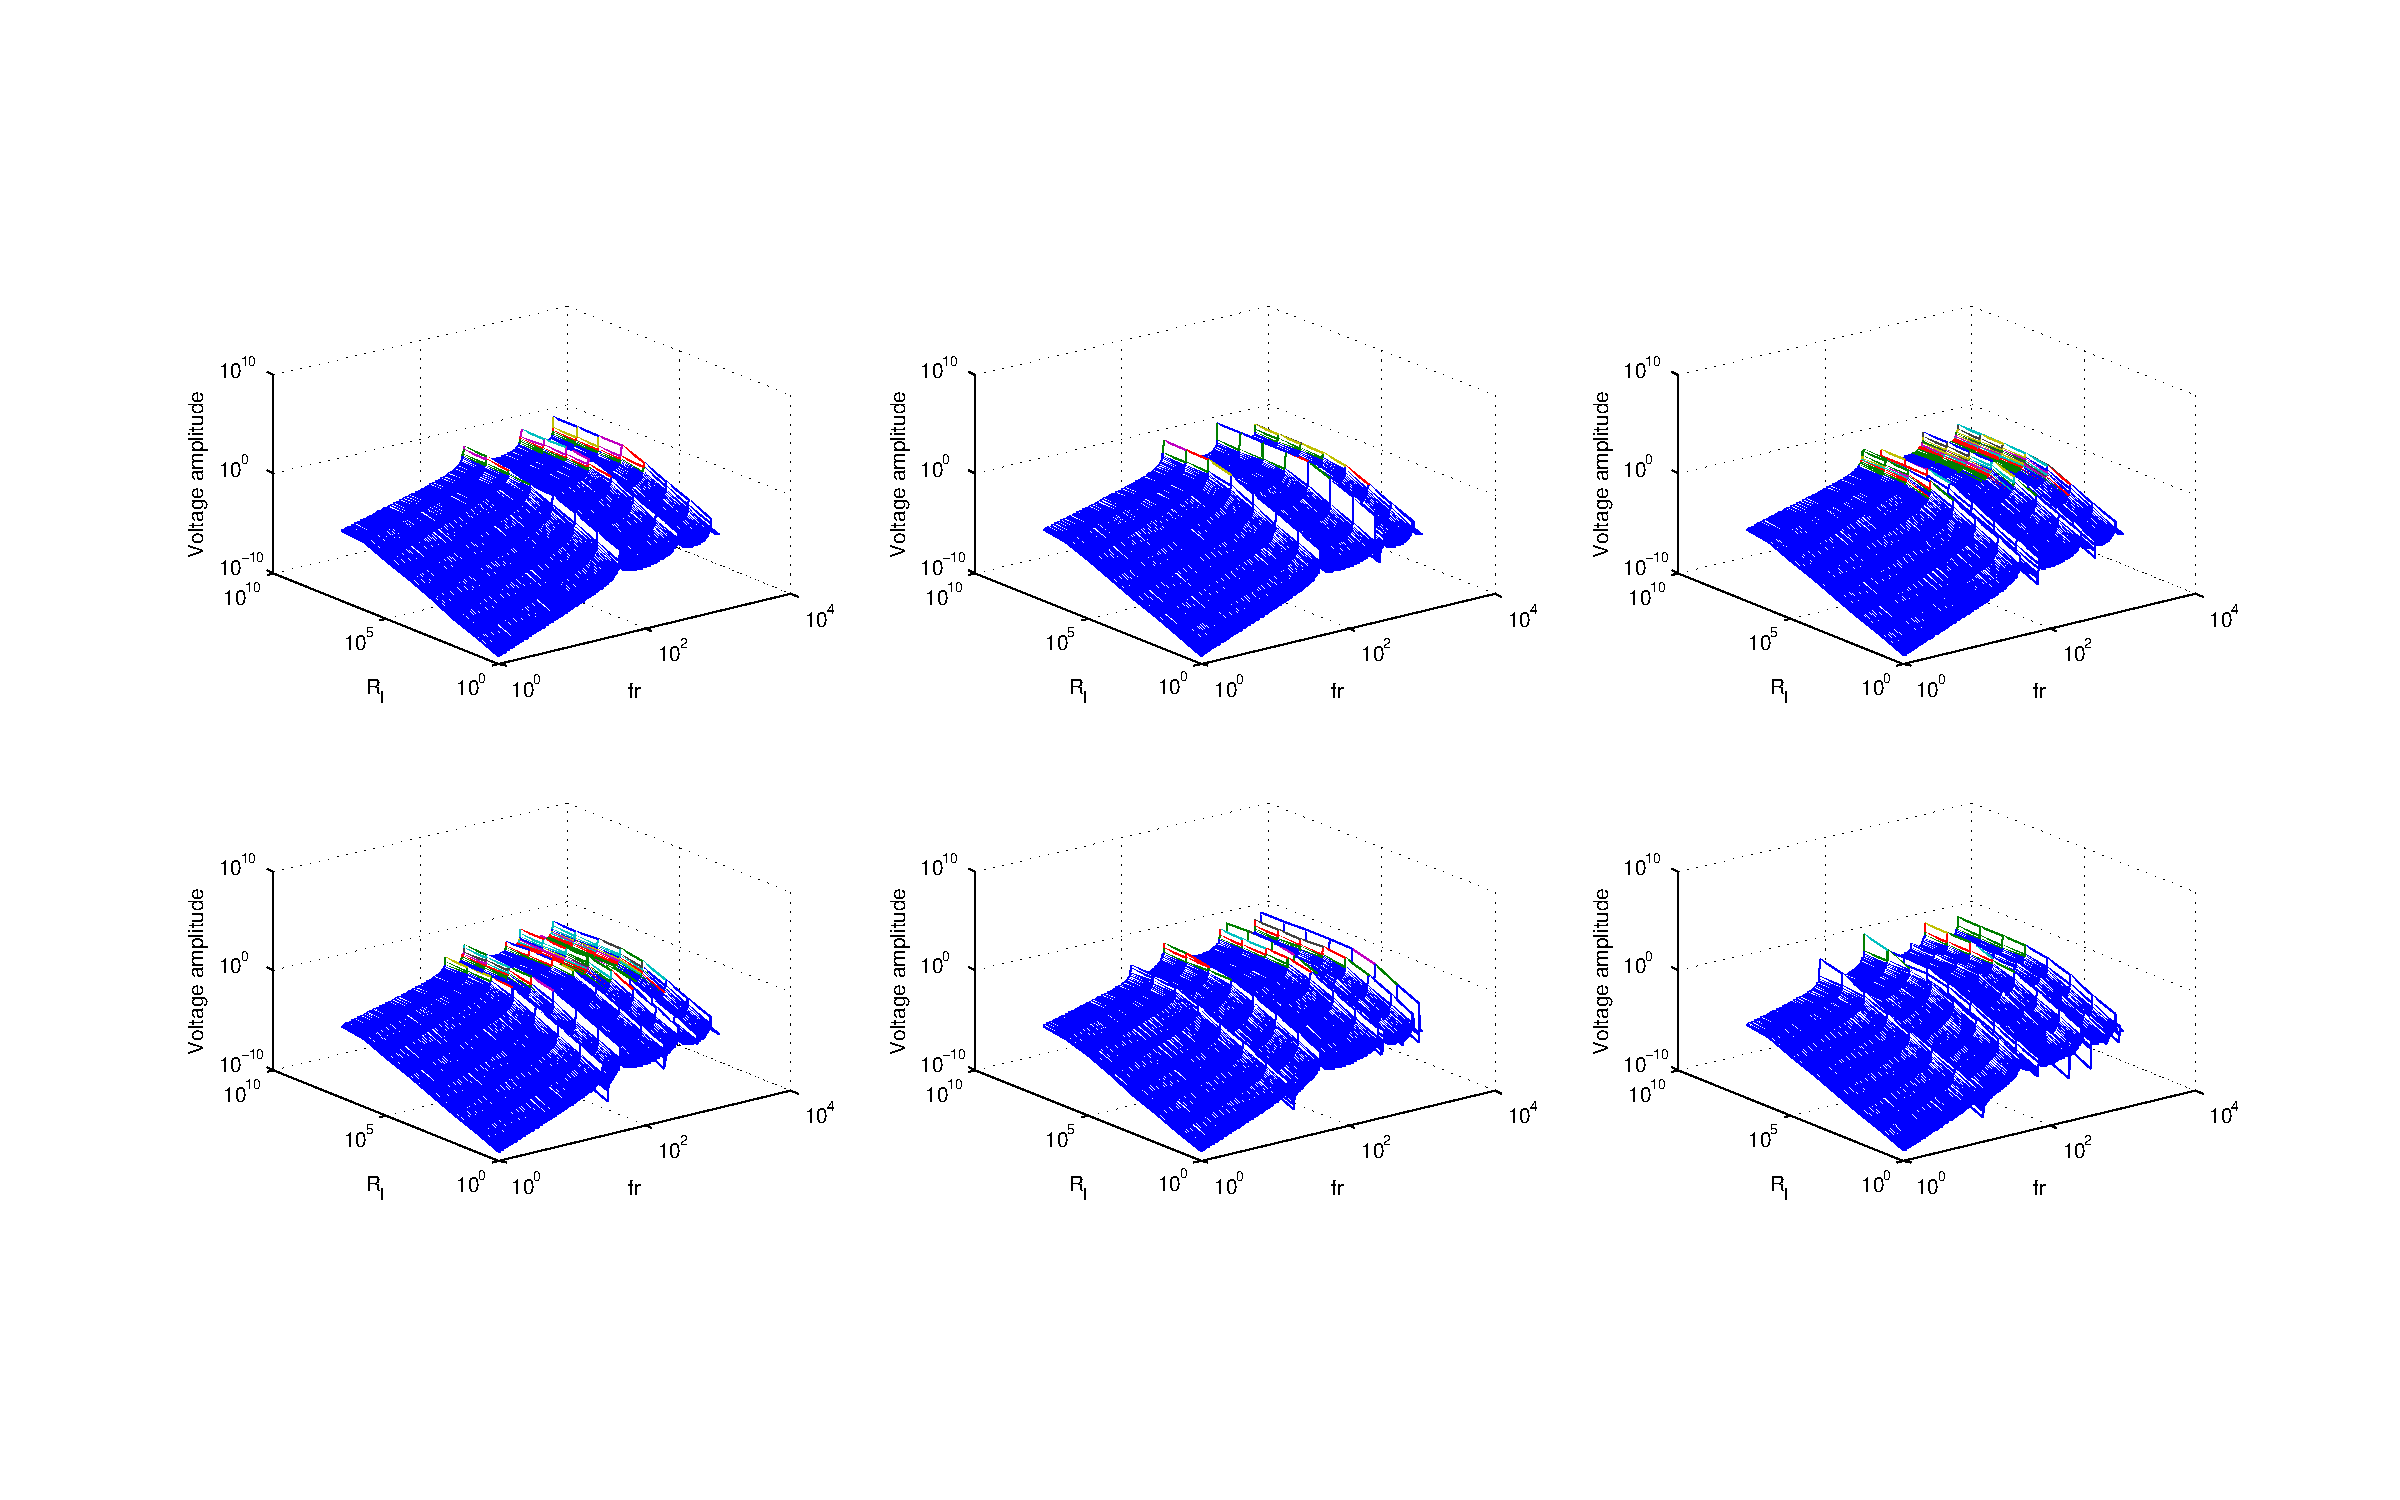
\includegraphics[width=0.6\textwidth]{./fig_output_voltage_vs_fr_Rl_laml_all}
    \caption{Output voltage $V_p$ (amplitude) of the piezoelectric energy harvester with flexible extension versus length ratio $\lambda_l$ at different frequency $f$ and load resistance $R_l$. }
    \label{fig:fig_output_voltage_vs_fr_Rl_laml_all}
\end{figure}

According to Figure~\ref{fig:fig_output_voltage_vs_fr_Rl_laml_all} and Figure~\ref{fig:fig_output_power_vs_fr_Rl_laml_all}, 

It is easily seen from the diagram that the change of extension length $l_e$ have a great influence on the frequency response of the piezoelectric energy harvester. At the given values of $\lambda_B$ and $\lambda_m$, the contained vibration modes in the frequency range considered does change with respect to
the length ratio $\lambda_l$. When $\lambda_l$ is relatively small, which is below $0.3$ in our case, no extra vibration modes can be found in the frequency range of $1\ - \ 100\ Hz$. Hence the energy harvesting performances of the proposed energy harvesters are similar to that of a pure cantilever beam piezoelectric energy harvester. (note: it will be better if I can compare the resonant energy harvesting performance in this case) With further increase of the length ratio $\lambda_l$, there begins to exist an extra resonant and anti-resonant mode in the considered frequency range. In this view, the change of length ratio actually expands the bandwidth of the energy harvesting performances. Even when the length ratio $\lambda_l =\ 1.0$, three resonant modes are found in the frequency range. The point to be noticed is the existence of anti-resonant mode, which largely narrows the bandwidth of the energy harvester. This accompanying characteristic is to be further investigated in the following research. 

\begin{figure}[!htbp]
    \centering
    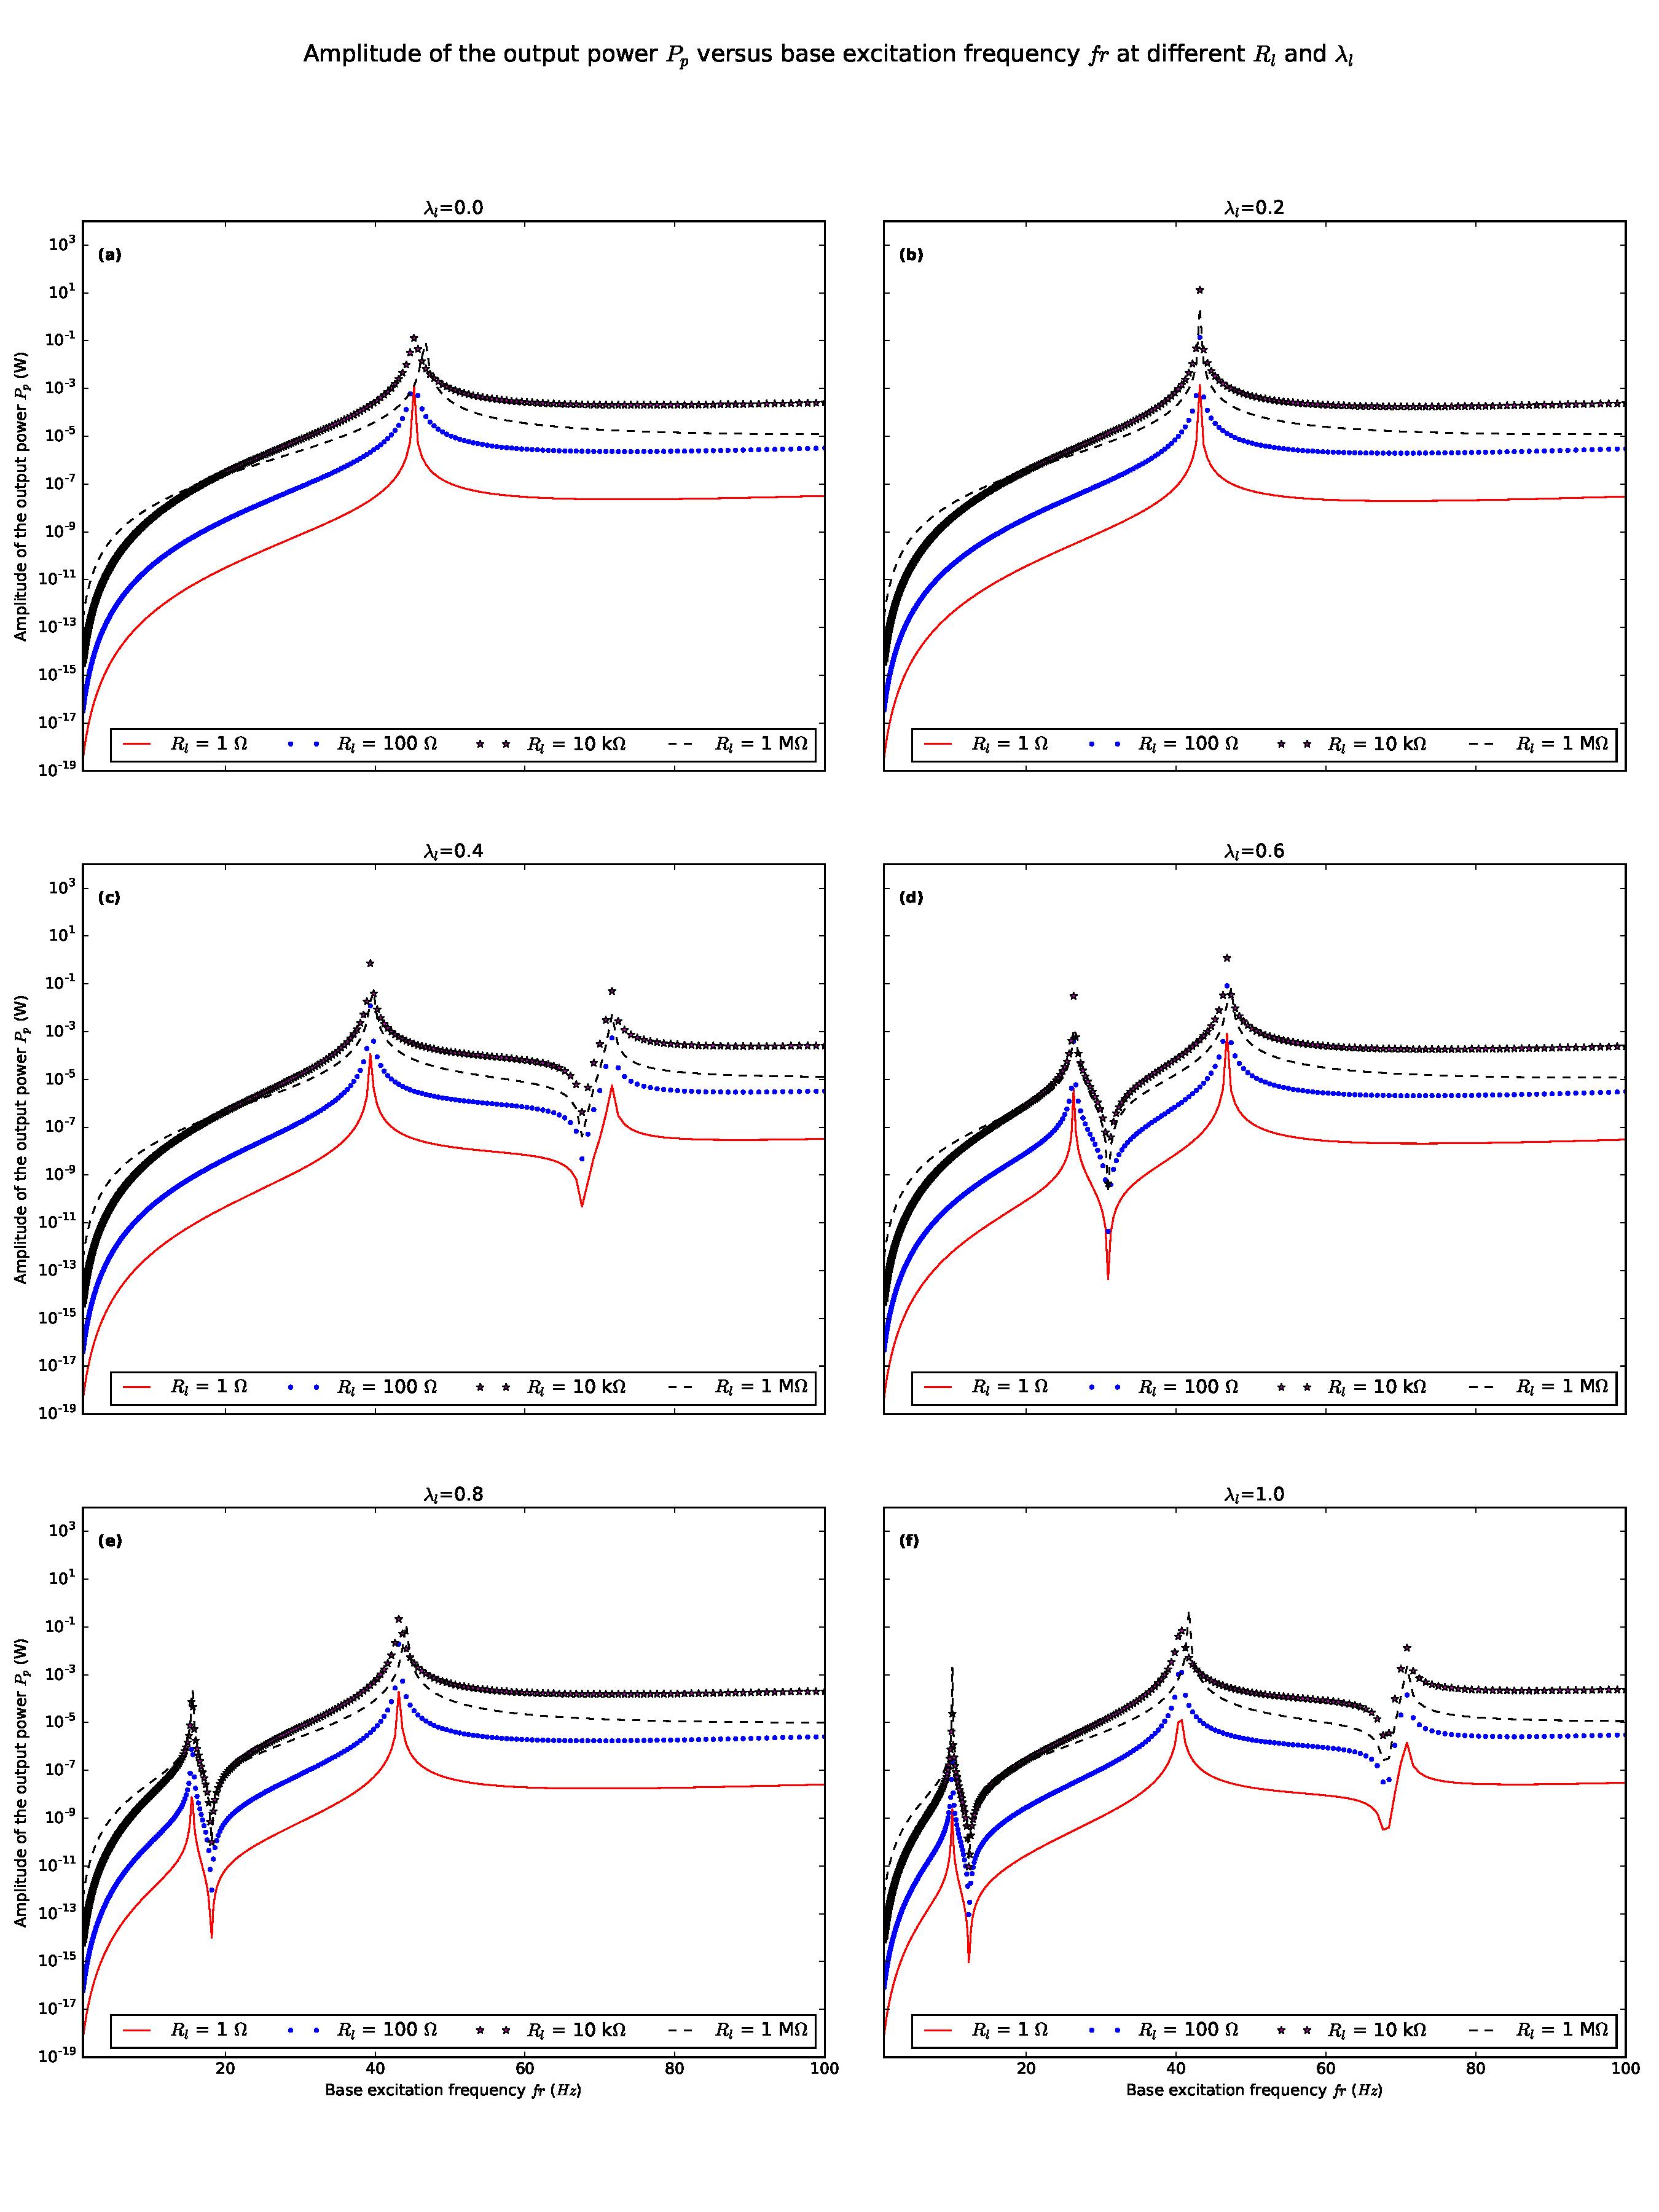
\includegraphics[width=0.6\textwidth]{./fig_output_power_vs_fr_Rl_laml_all}
    \caption{Output power $P_p$ (amplitude) of the piezoelectric energy harvester with flexible extension versus length ratio $\lambda_l$ at different frequency $f$ and load resistance $R_l$. }
    \label{fig:fig_output_power_vs_fr_Rl_laml_all}
\end{figure}


It is easily seen from the diagram that the change of extension length $l_e$ have a great influence on the frequency response of the piezoelectric energy harvester. At the given values of $\lambda_B$ and $\lambda_m$, the contained vibration modes in the frequency range considered does change with respect to
the length ratio $\lambda_l$. When $\lambda_l$ is relatively small, which is below $0.3$ in our case, no extra vibration modes can be found in the frequency range of $1\ - \ 100\ Hz$. Hence the energy harvesting performances of the proposed energy harvesters are similar to that of a pure cantilever beam piezoelectric energy harvester. (note: it will be better if I can compare the resonant energy harvesting performance in this case) With further increase of the length ratio $\lambda_l$, there begins to exist an extra resonant and anti-resonant mode in the considered frequency range. In this view, the change of length ratio actually expands the bandwidth of the energy harvesting performances. Even when the length ratio $\lambda_l =\ 1.0$, three resonant modes are found in the frequency range. The point to be noticed is the existence of anti-resonant mode, which largely narrows the bandwidth of the energy harvester. This accompanying characteristic is to be further investigated in the following research. 


\begin{figure}[!htbp]
    \centering
    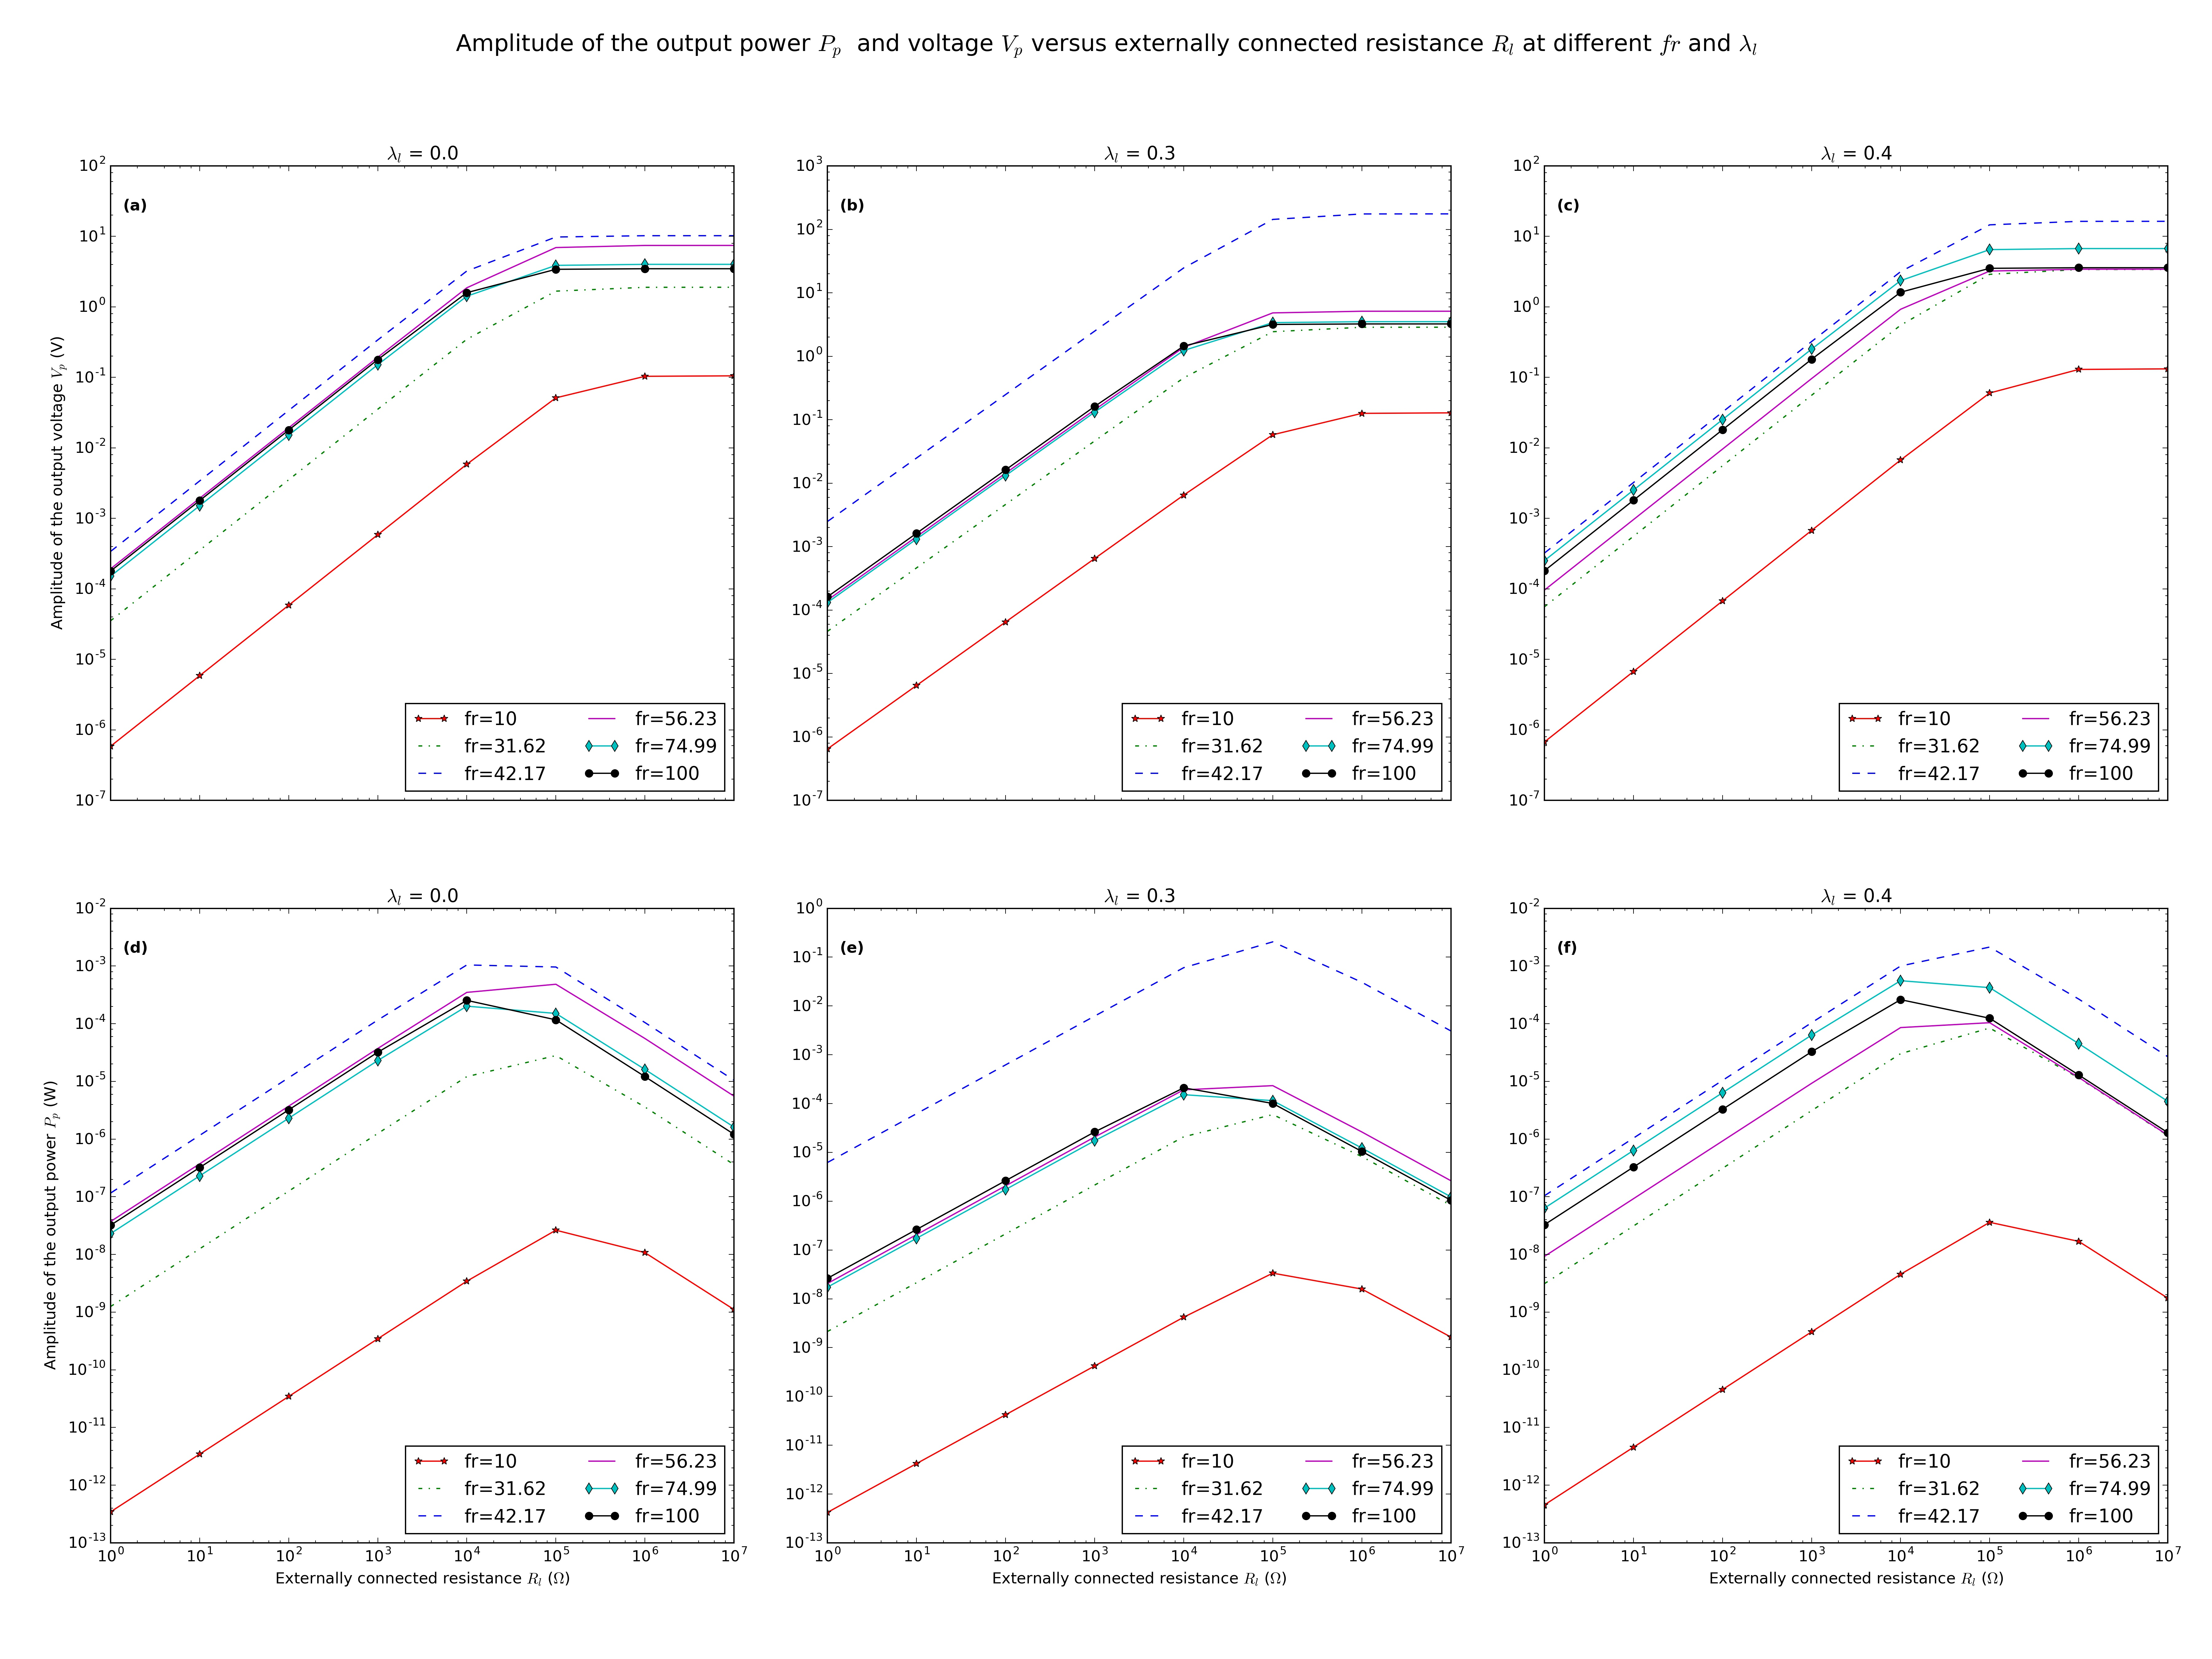
\includegraphics[width=0.6\textwidth]{./fig_perf_laml_0p3_0p4_vs_fr_Rl}
    \caption{Output voltage $V_p$ (amplitude) and output power $P_p$ (amplitude) of the piezoelectric energy harvester with flexible extension versus bending stiffness ratio $\lambda_l$ at different frequency $f$ and load resistance $R_l$. }
    \label{fig:fig_perf_laml_0p3_0p4_vs_fr_Rl}
\end{figure}

It is easily seen from the diagram that the change of extension length $l_e$ have a great influence on the frequency response of the piezoelectric energy harvester. At the given values of $\lambda_B$ and $\lambda_m$, the contained vibration modes in the frequency range considered does change with respect to
the length ratio $\lambda_l$. When $\lambda_l$ is relatively small, which is below $0.3$ in our case, no extra vibration modes can be found in the frequency range of $1\ - \ 100\ Hz$. Hence the energy harvesting performances of the proposed energy harvesters are similar to that of a pure cantilever beam piezoelectric energy harvester. (note: it will be better if I can compare the resonant energy harvesting performance in this case) With further increase of the length ratio $\lambda_l$, there begins to exist an extra resonant and anti-resonant mode in the considered frequency range. In this view, the change of length ratio actually expands the bandwidth of the energy harvesting performances. Even when the length ratio $\lambda_l =\ 1.0$, three resonant modes are found in the frequency range. The point to be noticed is the existence of anti-resonant mode, which largely narrows the bandwidth of the energy harvester. This accompanying characteristic is to be further investigated in the following research. 

\begin{figure}[!htbp]
    \centering
    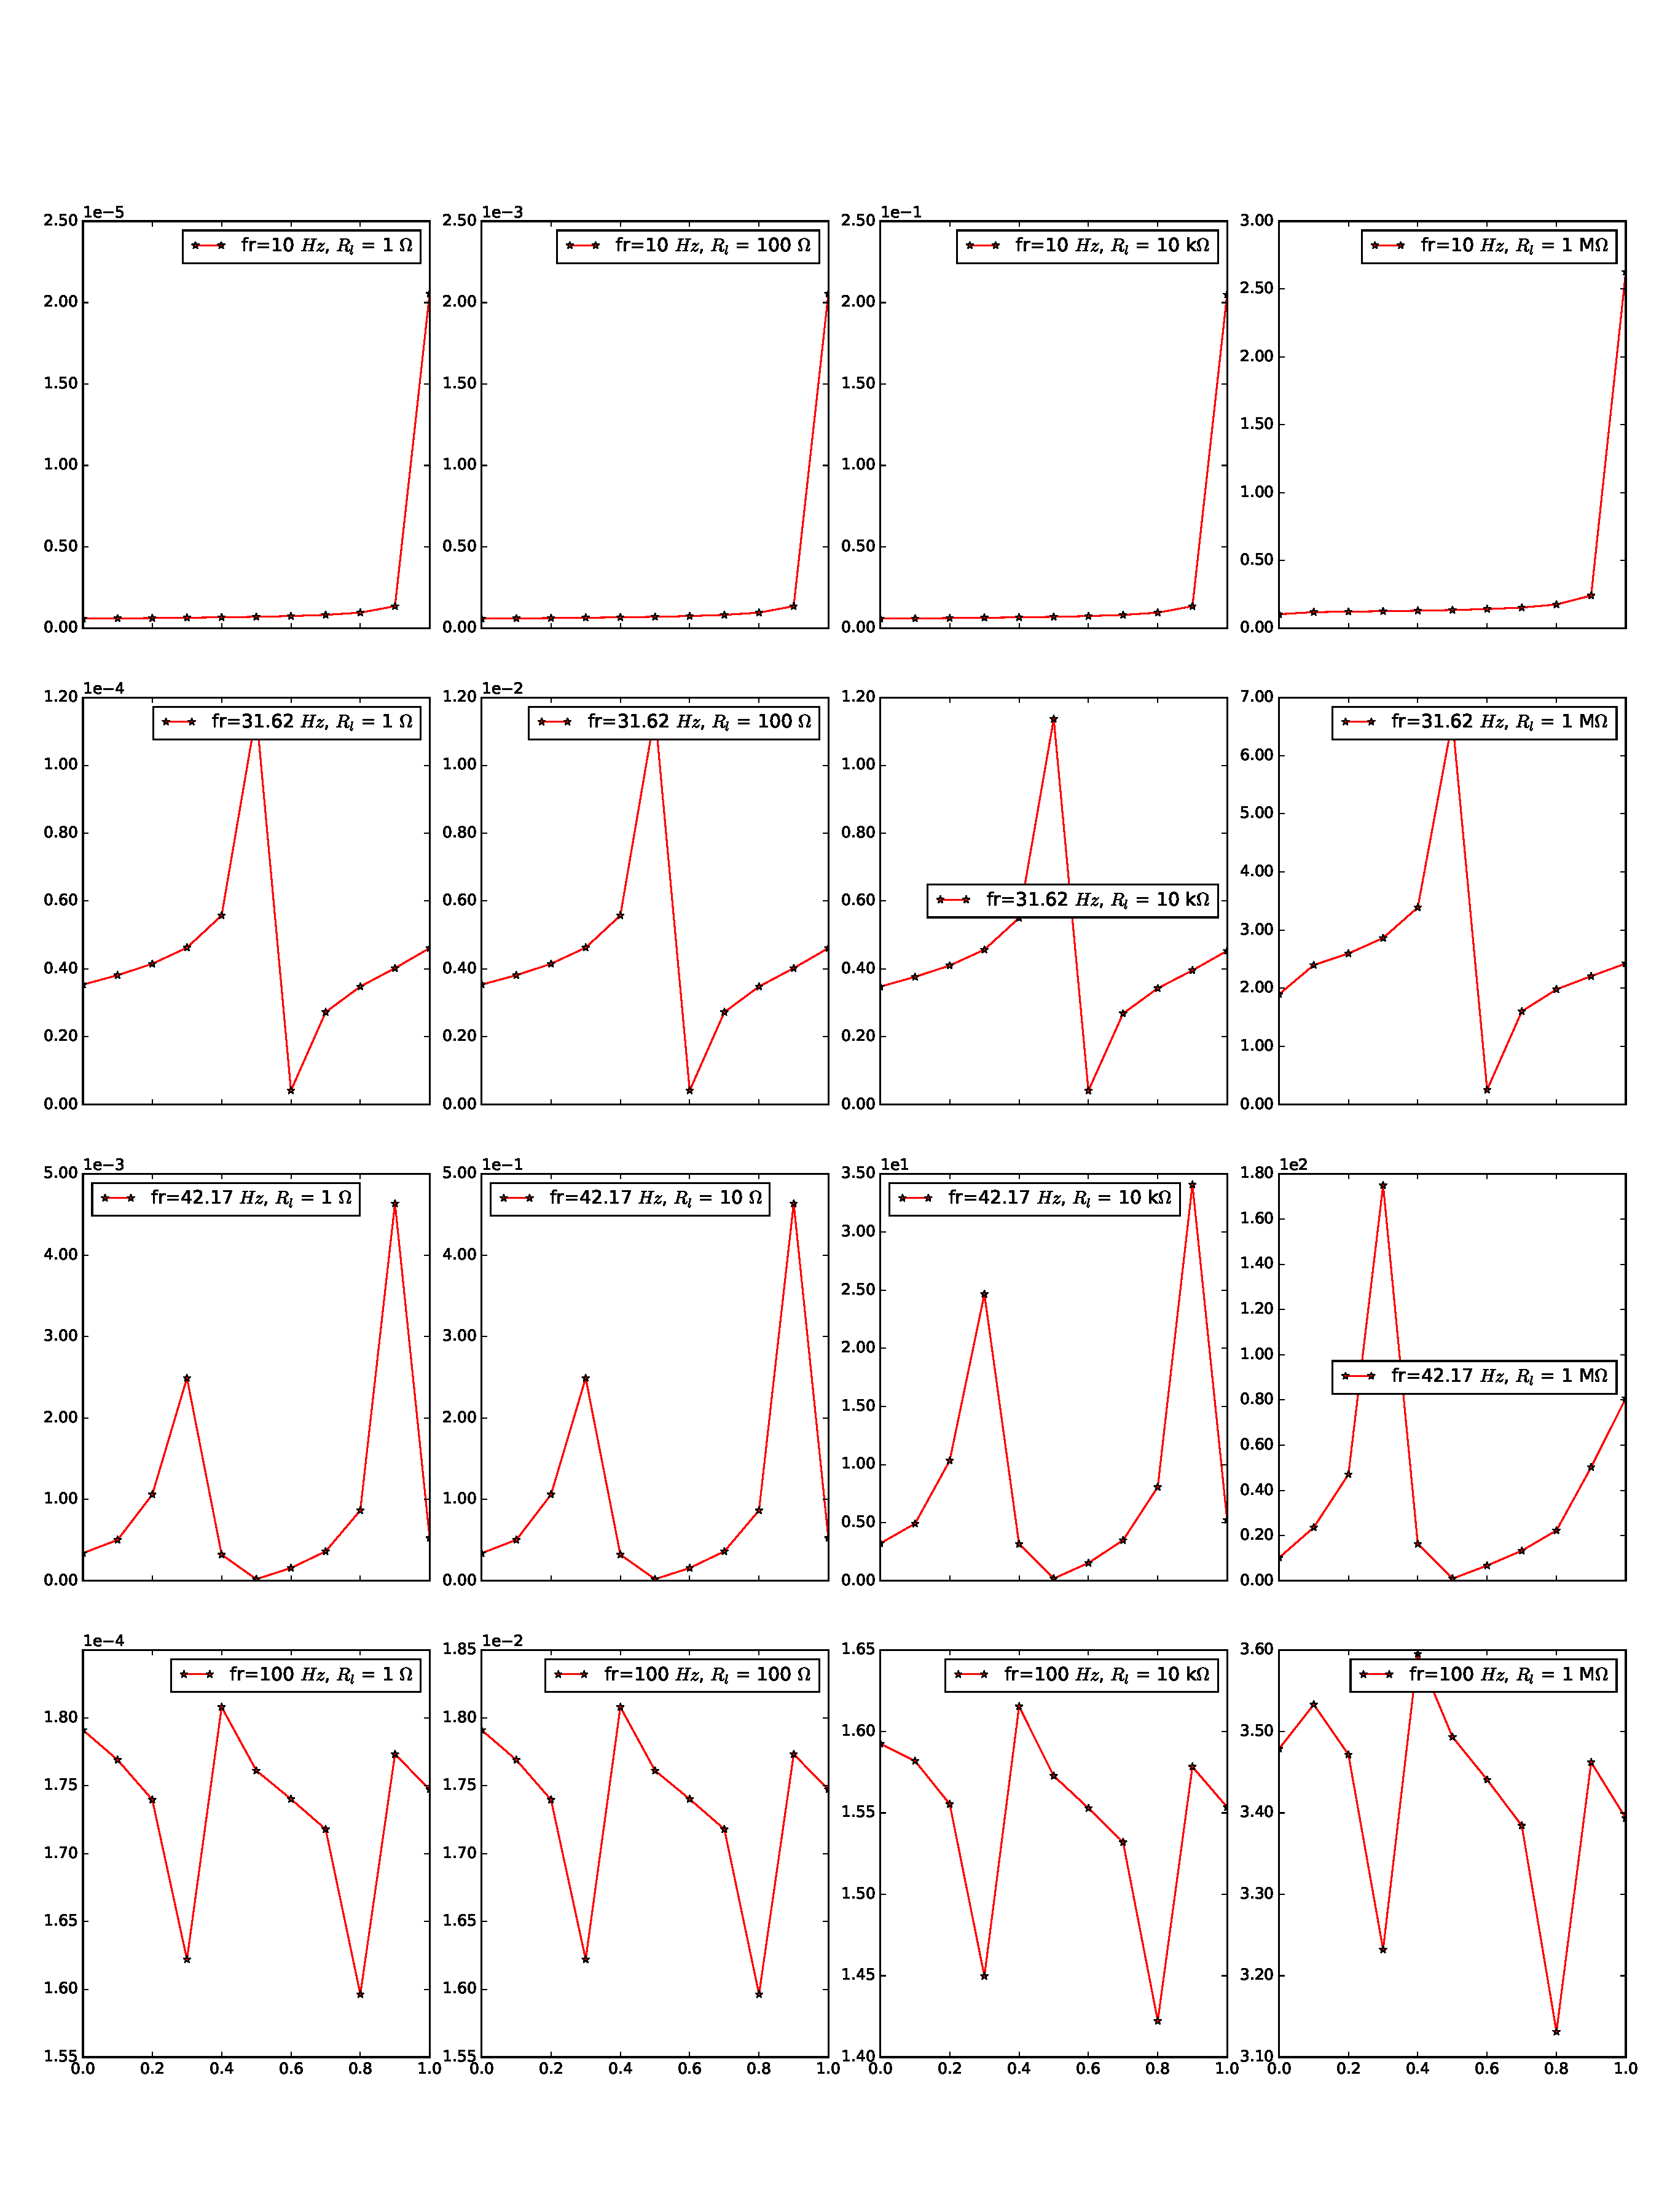
\includegraphics[width=0.6\textwidth]{./fig_vol_fr_sl_Rl_sl_vs_laml}
    \caption{Output voltage $V_p$ (amplitude) and output power $P_p$ (amplitude) of the piezoelectric energy harvester with flexible extension versus bending stiffness ratio $\lambda_l$ at different frequency $f$ and load resistance $R_l$. }
    \label{fig:fig_vol_fr_sl_Rl_sl_vs_laml}
\end{figure}

It is easily seen from the diagram that the change of extension length $l_e$ have a great influence on the frequency response of the piezoelectric energy harvester. At the given values of $\lambda_B$ and $\lambda_m$, the contained vibration modes in the frequency range considered does change with respect to
the length ratio $\lambda_l$. When $\lambda_l$ is relatively small, which is below $0.3$ in our case, no extra vibration modes can be found in the frequency range of $1\ - \ 100\ Hz$. Hence the energy harvesting performances of the proposed energy harvesters are similar to that of a pure cantilever beam piezoelectric energy harvester. (note: it will be better if I can compare the resonant energy harvesting performance in this case) With further increase of the length ratio $\lambda_l$, there begins to exist an extra resonant and anti-resonant mode in the considered frequency range. In this view, the change of length ratio actually expands the bandwidth of the energy harvesting performances. Even when the length ratio $\lambda_l =\ 1.0$, three resonant modes are found in the frequency range. The point to be noticed is the existence of anti-resonant mode, which largely narrows the bandwidth of the energy harvester. This accompanying characteristic is to be further investigated in the following research. 

\begin{figure}[!htbp]
    \centering
    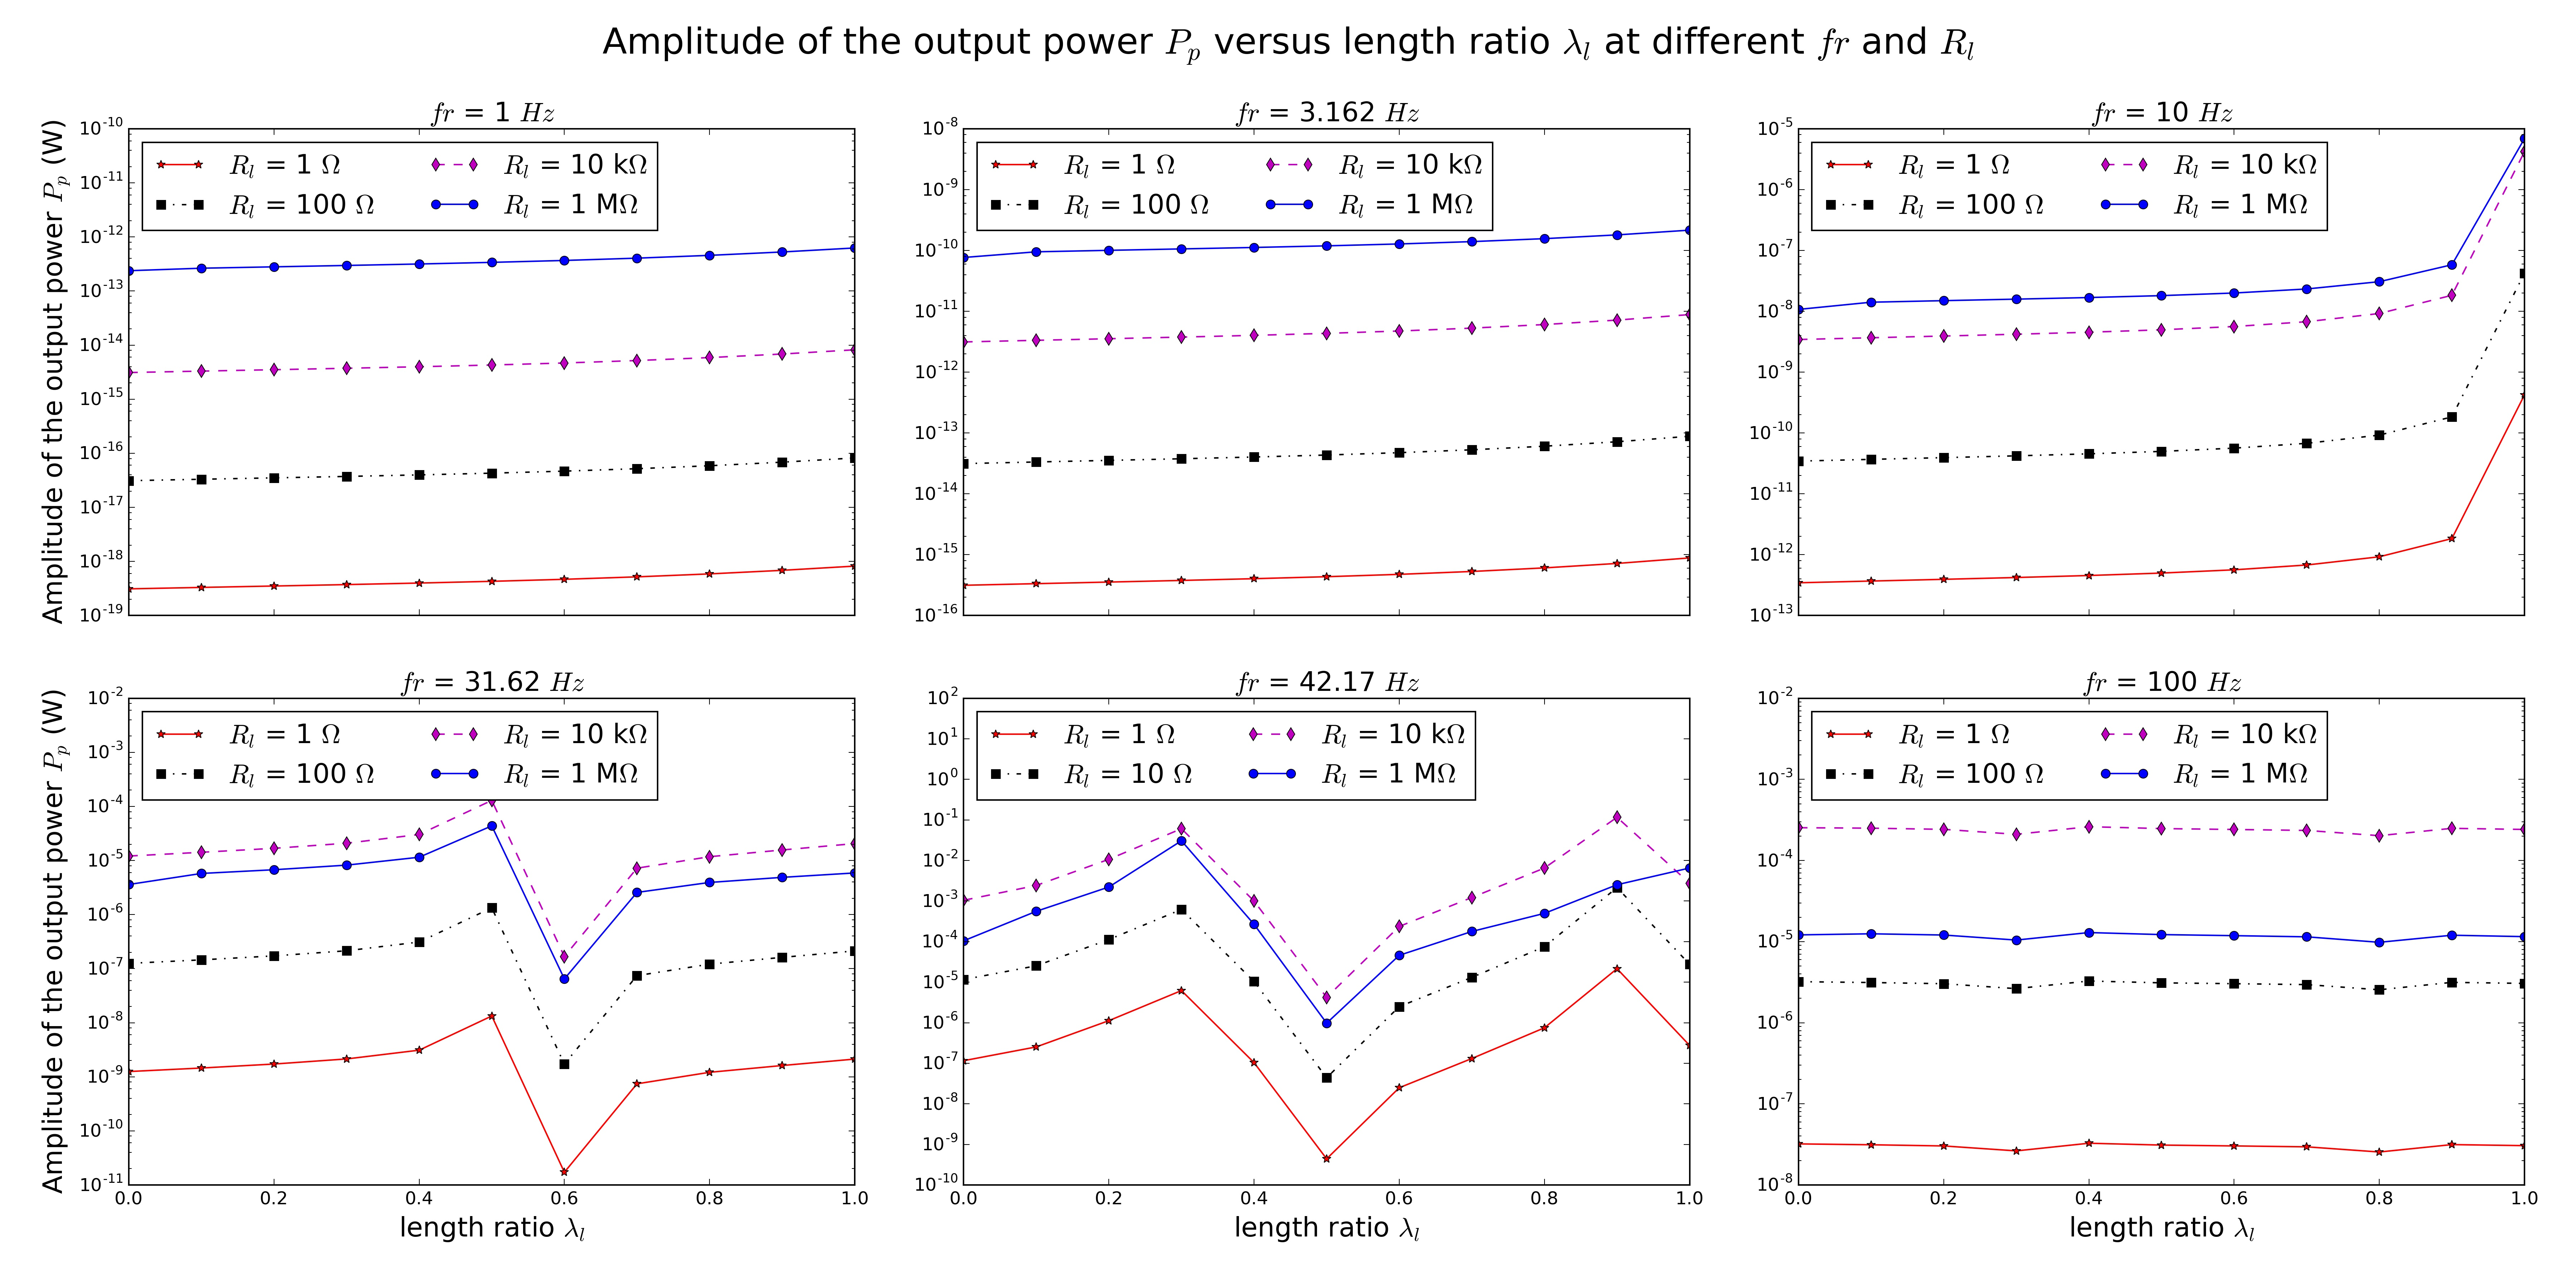
\includegraphics[width=0.6\textwidth]{./fig_pow_fr_sl_Rl_sl_vs_laml}
    \caption{Output voltage $V_p$ (amplitude) and output power $P_p$ (amplitude) of the piezoelectric energy harvester with flexible extension versus bending stiffness ratio $\lambda_l$ at different frequency $f$ and load resistance $R_l$. }
    \label{fig:fig_pow_fr_sl_Rl_sl_vs_laml}
\end{figure}


\subsection{beam extension bending stiffness or bending stiffness ratio $\lambda_B$}


\begin{figure}[!htbp]
    \centering
    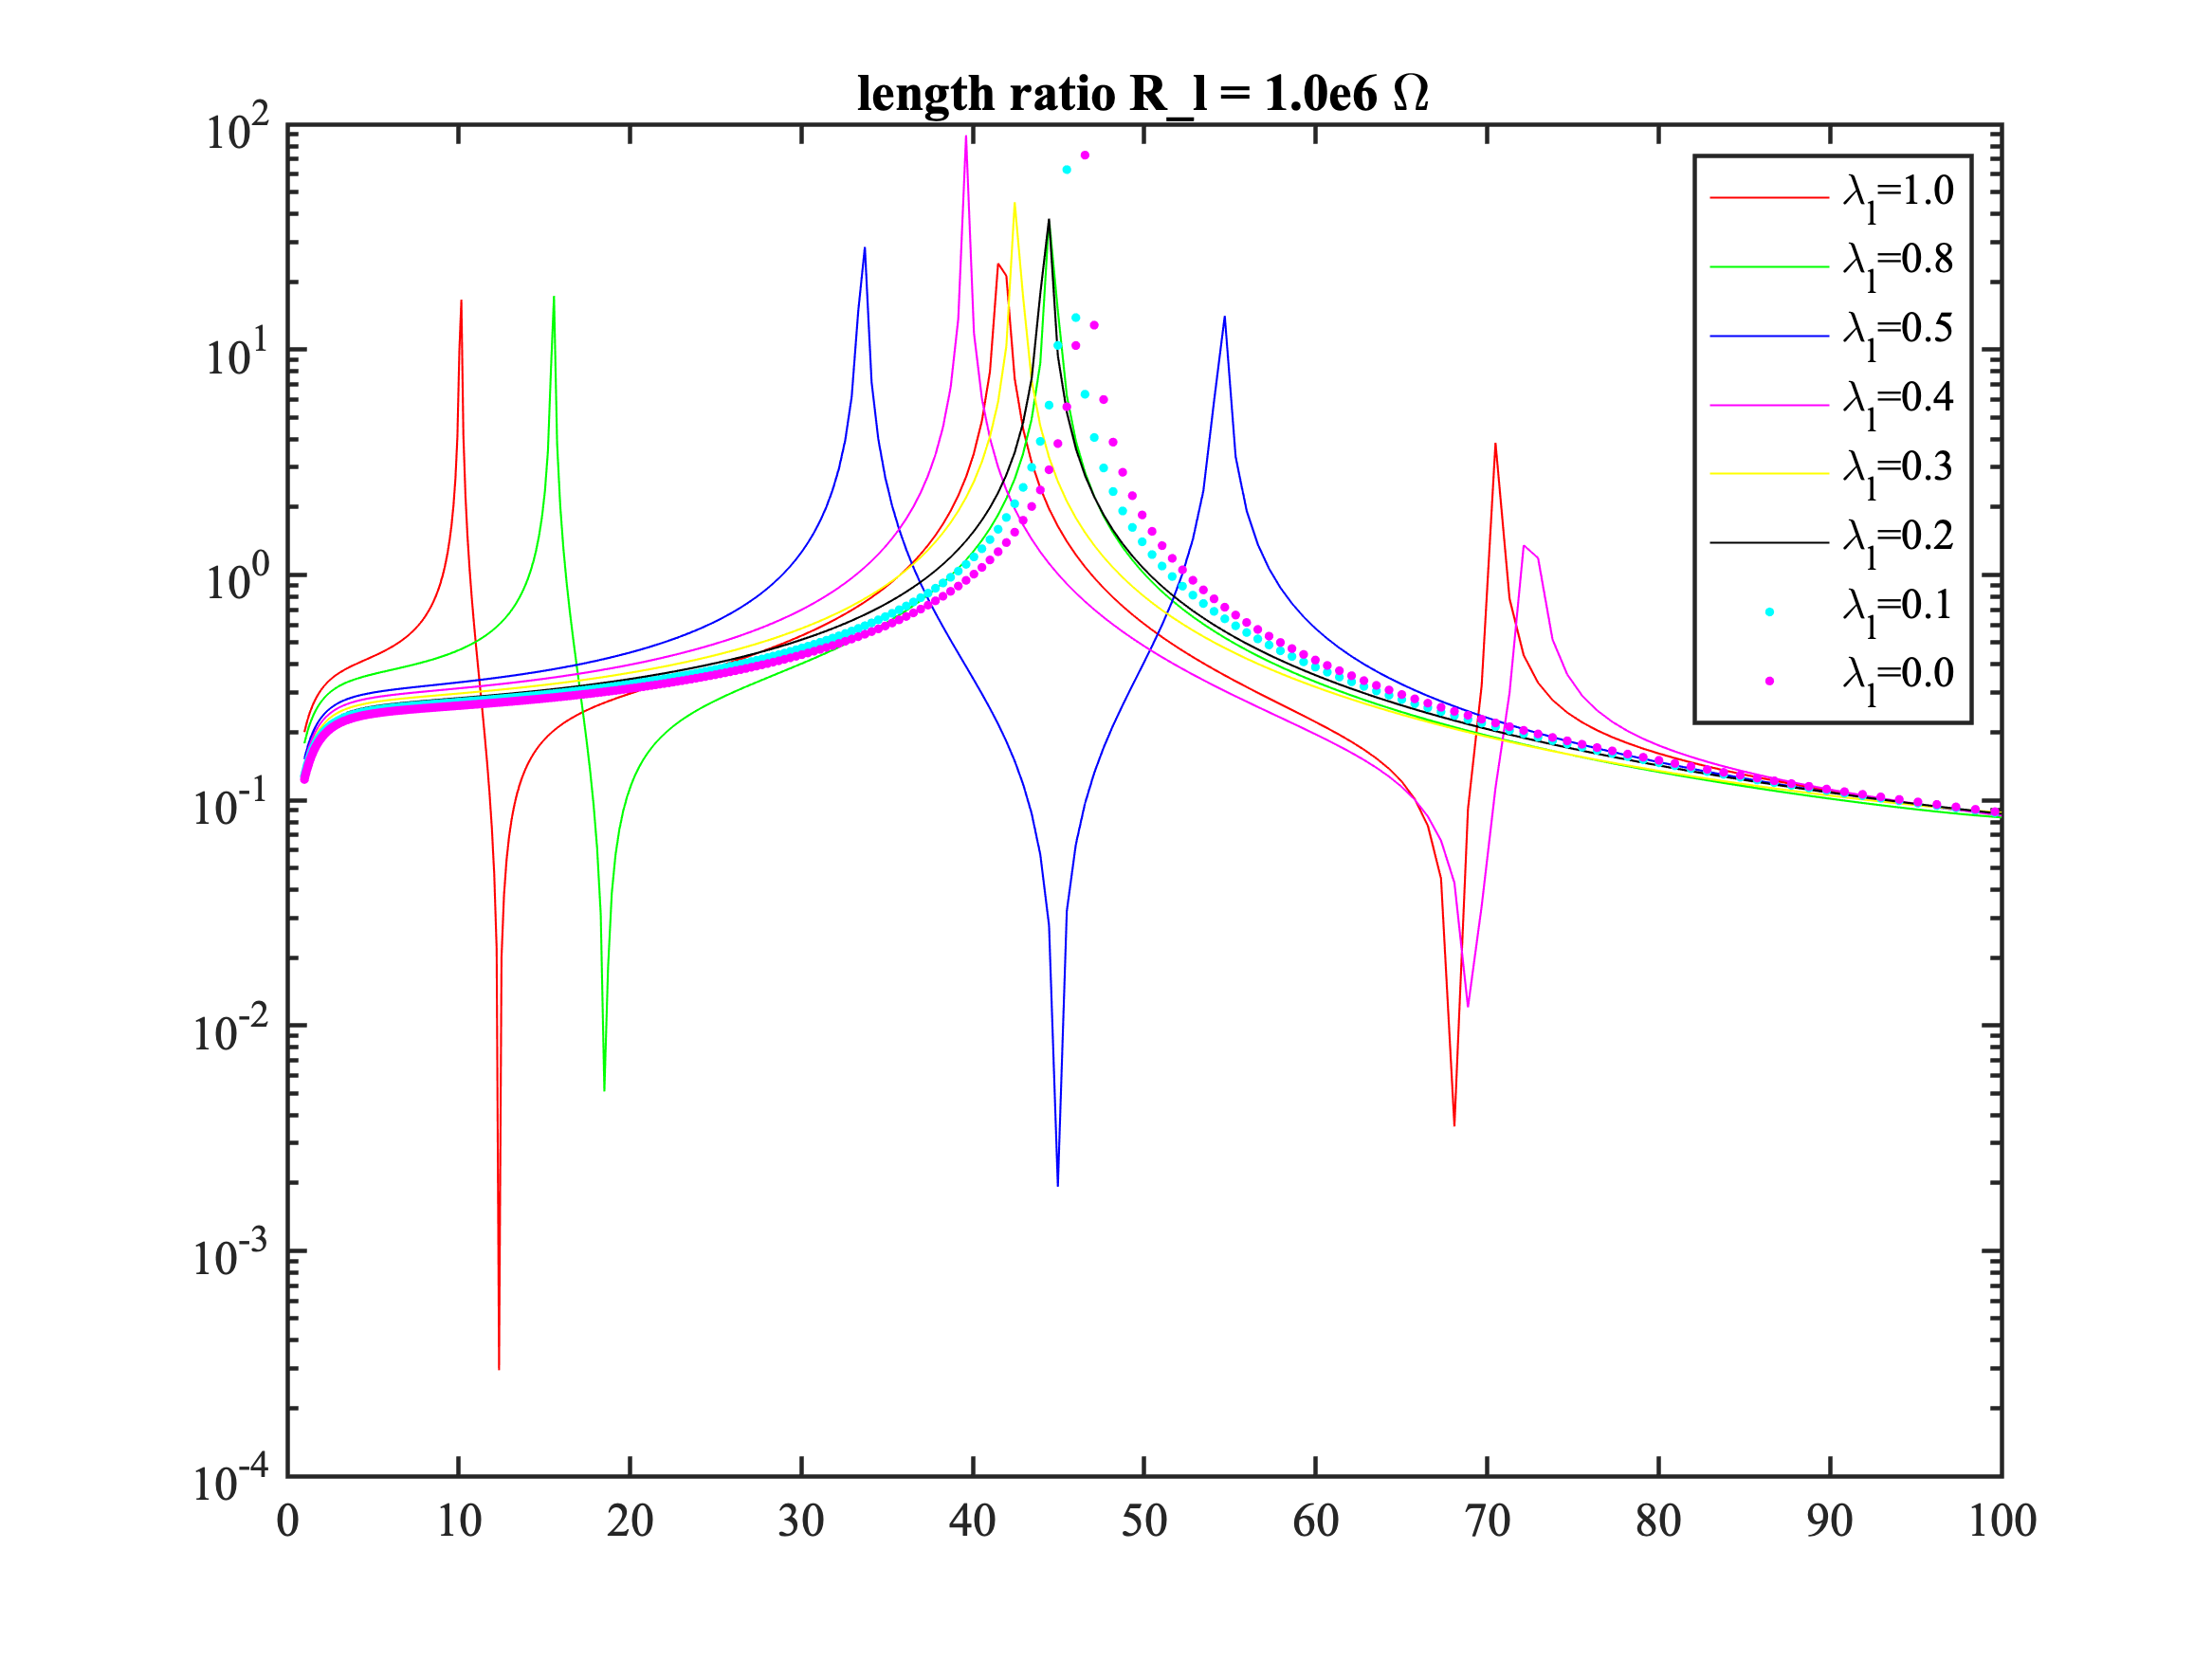
\includegraphics[width=0.6\textwidth]{./fig_laml_vol_versus_fr_Rl}
    \caption{Output voltage $V_p$ (amplitude) and output power $P_p$ (amplitude) of the piezoelectric energy harvester with flexible extension versus bending stiffness ratio $\lambda_l$ at different frequency $f$ and load resistance $R_l$. }
    \label{fig:fig_lamB_vol_versus_fr_Rl}
\end{figure}

It is easily seen from the diagram that the change of extension length $l_e$ have a great influence on the frequency response of the piezoelectric energy harvester. At the given values of $\lambda_B$ and $\lambda_m$, the contained vibration modes in the frequency range considered does change with respect to
the length ratio $\lambda_l$. When $\lambda_l$ is relatively small, which is below $0.3$ in our case, no extra vibration modes can be found in the frequency range of $1\ - \ 100\ Hz$. Hence the energy harvesting performances of the proposed energy harvesters are similar to that of a pure cantilever beam piezoelectric energy harvester. (note: it will be better if I can compare the resonant energy harvesting performance in this case) With further increase of the length ratio $\lambda_l$, there begins to exist an extra resonant and anti-resonant mode in the considered frequency range. In this view, the change of length ratio actually expands the bandwidth of the energy harvesting performances. Even when the length ratio $\lambda_l = 1.0$, three resonant modes are found in the frequency range. The point to be noticed is the existence of anti-resonant mode, which largely narrows the bandwidth of the energy harvester. This accompanying characteristic is to be further investigated in the following research. 



\subsection{beam extension line density or line density ratio $\lambda_m$}


\begin{figure}[!htbp]
    \centering
    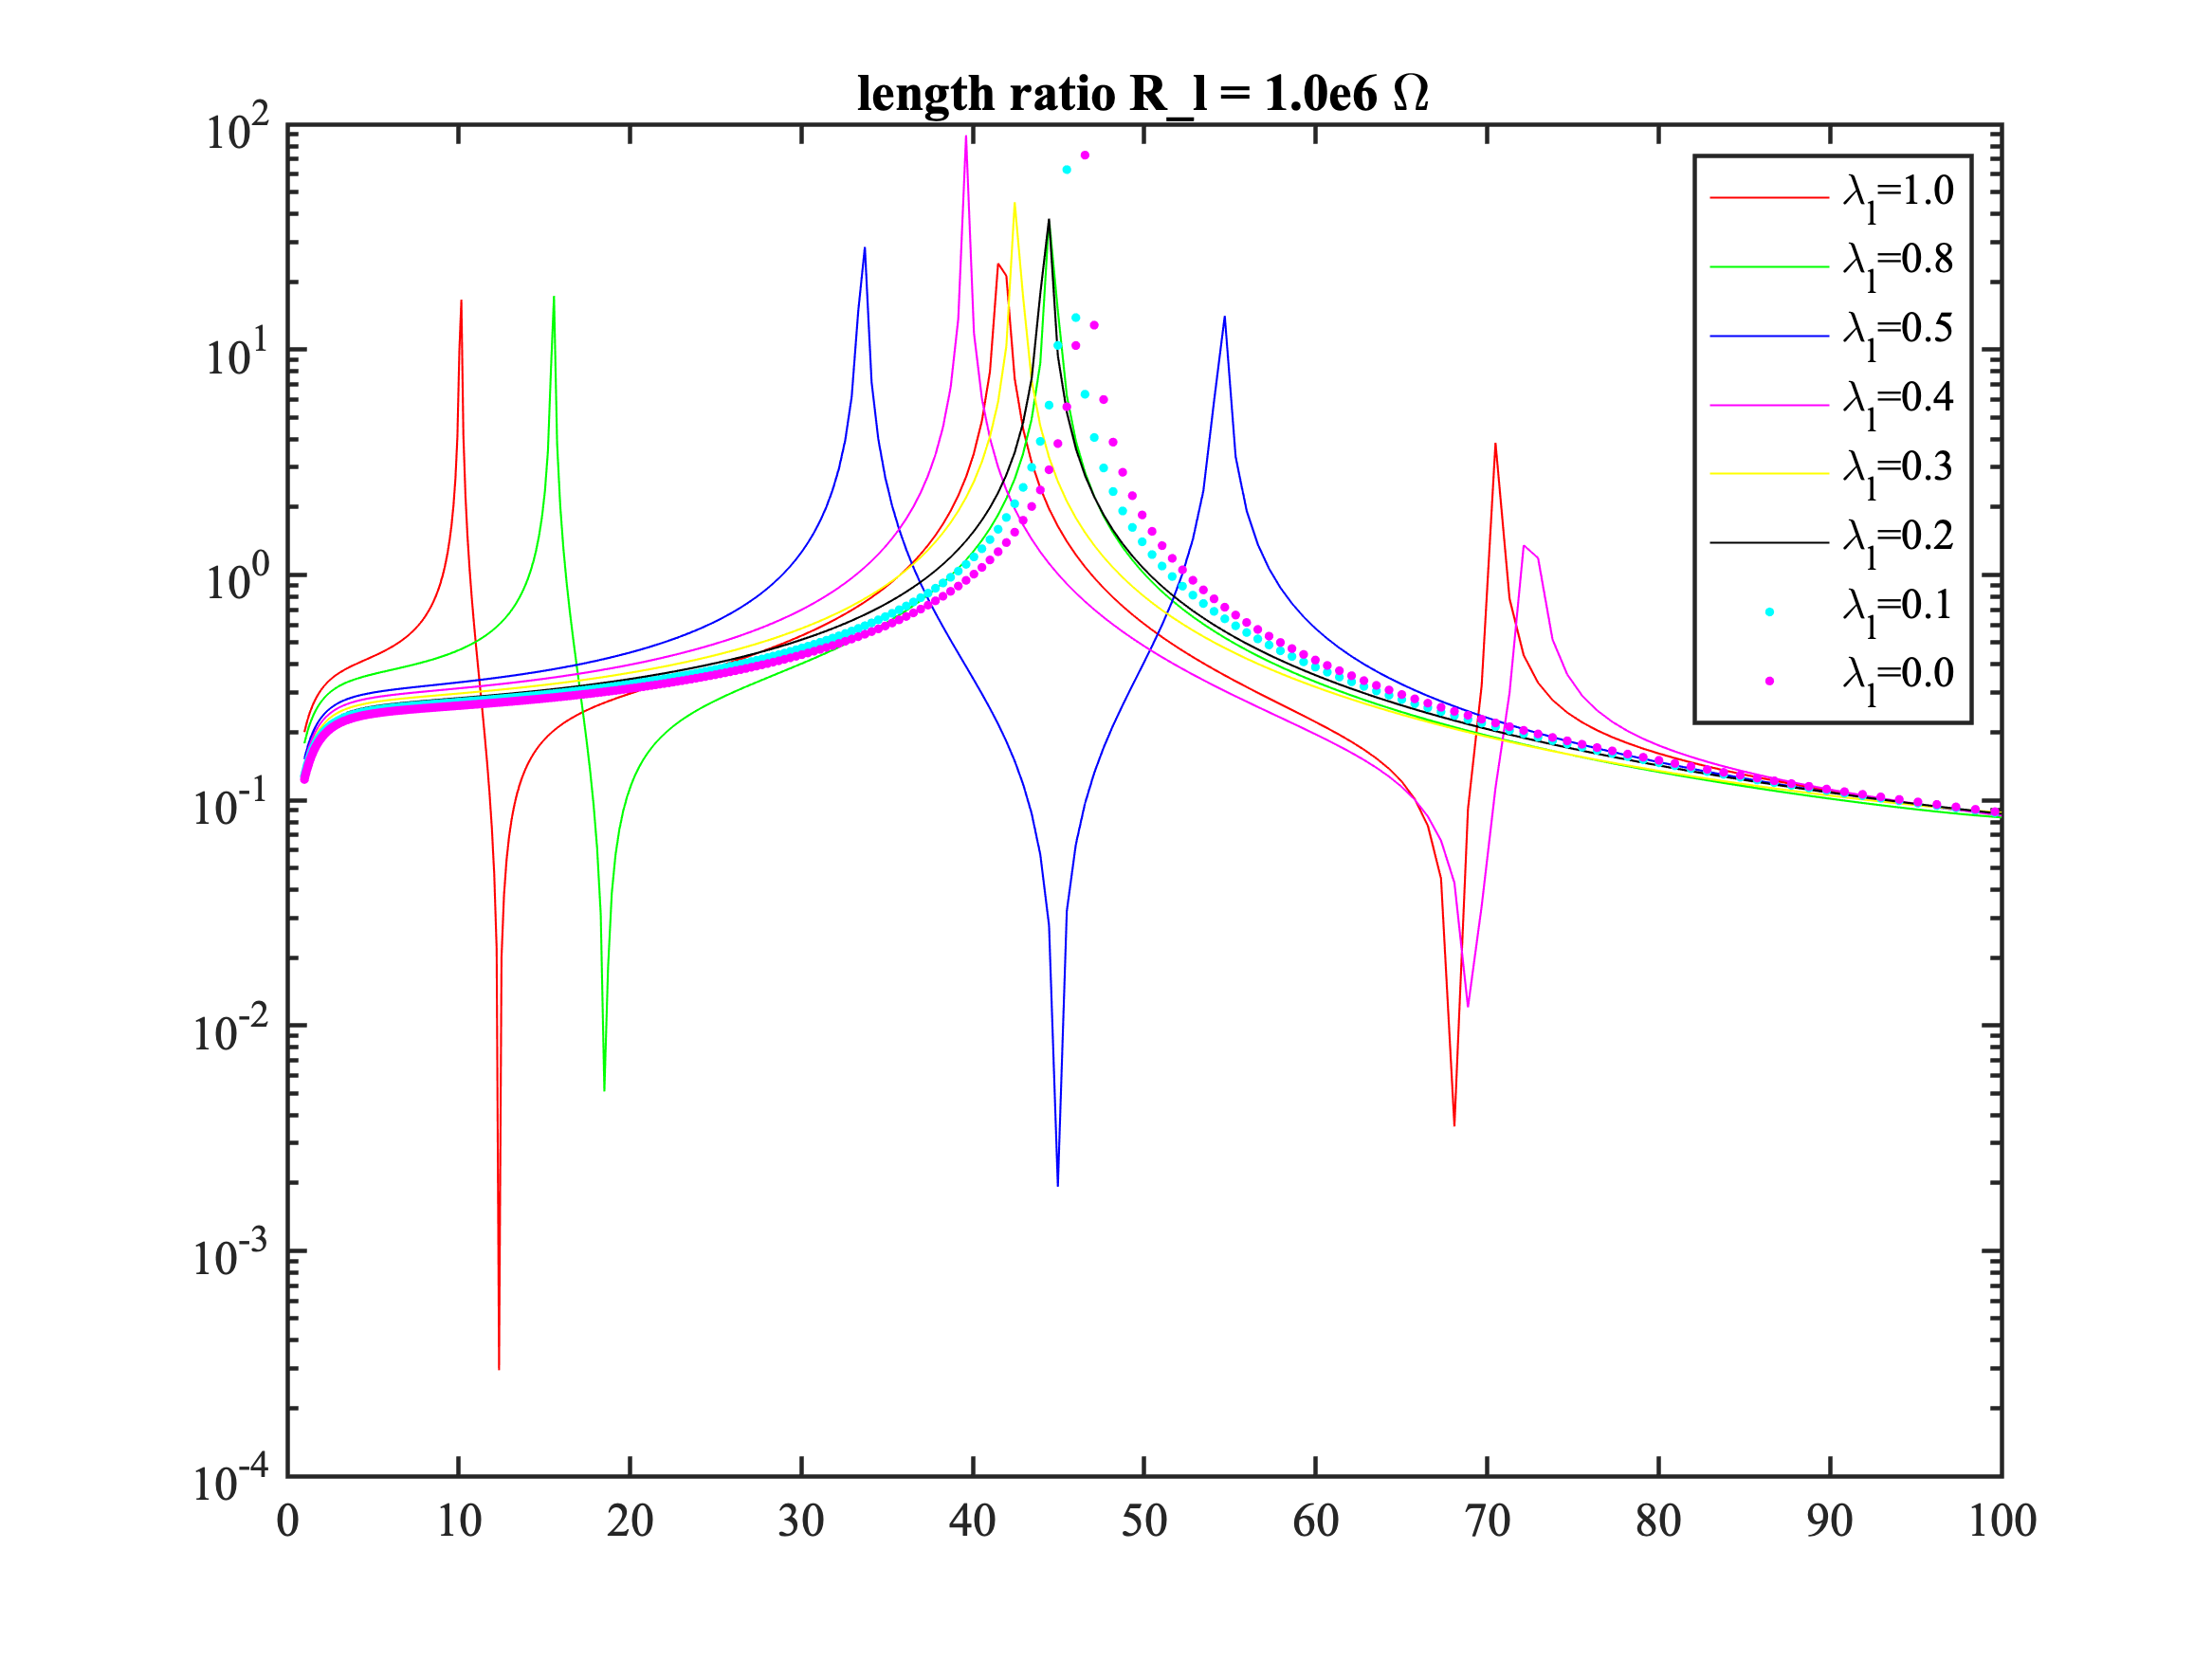
\includegraphics[width=0.6\textwidth]{./fig_laml_vol_versus_fr_Rl}
    \caption{Output voltage $V_p$ (amplitude) and output power $P_p$ (amplitude) of the piezoelectric energy harvester with flexible extension versus line mass density ratio $\lambda_m$ at different frequency $f$ and load resistance $R_l$. }
    \label{fig:fig_lamm_vol_versus_fr_Rl}
\end{figure}

It is easily seen from the diagram that the change of extension length $l_e$ have a great influence on the frequency response of the piezoelectric energy harvester. At the given values of $\lambda_B$ and $\lambda_m$, the contained vibration modes in the frequency range considered does change with respect to
the length ratio $\lambda_l$. When $\lambda_l$ is relatively small, which is below $0.3$ in our case, no extra vibration modes can be found in the frequency range of $1\ - \ 100\ Hz$. Hence the energy harvesting performances of the proposed energy harvesters are similar to that of a pure cantilever beam piezoelectric energy harvester. (note: it will be better if I can compare the resonant energy harvesting performance in this case) With further increase of the length ratio $\lambda_l$, there begins to exist an extra resonant and anti-resonant mode in the considered frequency range. In this view, the change of length ratio actually expands the bandwidth of the energy harvesting performances. Even when the length ratio $\lambda_l = 1.0$, three resonant modes are found in the frequency range. The point to be noticed is the existence of anti-resonant mode, which largely narrows the bandwidth of the energy harvester. This accompanying characteristic is to be further investigated in the following research. 


\section{Discussion}



\section{Conclusion}

Here in this contribution, we investigate the method of flexible extension to tune the energy harvesting performance of piezoelectric cantilever energy harvester.


\section*{Reference}

\bibliography{maureenchou.bib}
\bibliographystyle{vancouver}


\end{document}



% The conservation of momentum and inextensibility condition for the piezoelectric composite part lead to
% \begin{equation}
%   \begin{aligned}
%       \mu \frac{\partial^2 \mathbf{X}}{\partial T^2} &= \frac{\partial}{\partial S} \left[ F_T \mathbf{e}_\tau - F_N \mathbf{e}_n \right] \\
%       \frac{\partial M}{\partial S} &= F_N \\
%       \frac{\partial \mathbf{X}}{\partial S} &= \mathbf{e}_\tau
%   \end{aligned}
% \end{equation}
% As a result, we have
% \begin{equation}
%   \begin{aligned}
%       \mu \frac{\partial^2 \mathbf{X}}{\partial T^2} &= \frac{\partial}{\partial S} \left[ F_T \mathbf{e}_\tau - \frac{\partial M}{\partial S} \mathbf{e}_n \right] \\
%       \frac{\partial \mathbf{X}}{\partial S} &= \mathbf{e}_\tau
%   \end{aligned}
% \end{equation}